\documentclass[a4paper]{article}
%%%%%%%%%%%%%%%%%%%%%%%%%%%%%%%%%%%%%%%%%%
%  My documentation report
%  Objetive: Explain what I did and how, so someone can continue with the investigation
%
% Important note:
% Chapter heading images should have a 2:1 width:height ratio,
% e.g. 920px width and 460px height.
%
%%%%%%%%%%%%%%%%%%%%%%%%%%%%%%%%%%%%%%%%%


%----------------------------------------------------------------------------------------
%	PACKAGES AND OTHER DOCUMENT CONFIGURATIONS
%----------------------------------------------------------------------------------------

\documentclass[11pt,fleqn]{book} % Default font size and left-justified equations

\usepackage[top=3cm,bottom=3cm,left=3.2cm,right=3.2cm,headsep=10pt,letterpaper]{geometry} % Page margins

\usepackage{xcolor} % Required for specifying colors by name
\definecolor{ocre}{RGB}{52,177,201} % Define the orange color used for highlighting throughout the book
\usepackage{graphicx}
\usepackage{wrapfig}
% Font Settings
\usepackage{avant} % Use the Avantgarde font for headings
%\usepackage{times} % Use the Times font for headings
\usepackage{mathptmx} % Use the Adobe Times Roman as the default text font together with math symbols from the Sym­bol, Chancery and Com­puter Modern fonts
\usepackage{microtype} % Slightly tweak font spacing for aesthetics
\usepackage[utf8]{inputenc} % Required for including letters with accents
\usepackage[T2A]{fontenc} % Use 8-bit encoding that has 256 glyphs
\usepackage[english,russian]{babel}
\usepackage{amsthm}
\usepackage{xcolor}

% Bibliography
\usepackage[style=alphabetic,sorting=nyt,sortcites=true,autopunct=true,=hyphen,hyperref=true,abbreviate=false,backref=true,backend=biber]{biblatex}
\addbibresource{bibliography.bib}
\defbibheading{bibempty}{}

%----------------------------------------------------------------------------------------
%	VARIOUS REQUIRED PACKAGES
%----------------------------------------------------------------------------------------

\usepackage{titlesec} % Allows customization of titles

\usepackage{graphicx} % Required for including pictures
\graphicspath{{Pictures/}} % Specifies the directory where pictures are stored
% \graphicspath{{Plots/}}
\usepackage{lipsum} % Inserts dummy text

\usepackage{tikz} % Required for drawing custom shapes

\usepackage[english]{babel} % English language/hyphenation

\usepackage{enumitem} % Customize lists
\setlist{nolistsep} % Reduce spacing between bullet points and numbered lists

\usepackage{booktabs} % Required for nicer horizontal rules in tables

\usepackage{eso-pic} % Required for specifying an image background in the title page

%----------------------------------------------------------------------------------------
%	MAIN TABLE OF CONTENTS
%----------------------------------------------------------------------------------------

\usepackage{titletoc} % Required for manipulating the table of contents

\contentsmargin{0cm} % Removes the default margin
% Chapter text styling
\titlecontents{chapter}[1.25cm] % Indentation
{\addvspace{15pt}\large\sffamily\bfseries} % Spacing and font options for chapters
{\color{ocre!60}\contentslabel[\Large\thecontentslabel]{1.25cm}\color{ocre}} % Chapter number
{}  
{\color{ocre!60}\normalsize\sffamily\bfseries\;\titlerule*[.5pc]{.}\;\thecontentspage} % Page number
% Section text styling
\titlecontents{section}[1.25cm] % Indentation
{\addvspace{5pt}\sffamily\bfseries} % Spacing and font options for sections
{\contentslabel[\thecontentslabel]{1.25cm}} % Section number
{}
{\sffamily\hfill\color{black}\thecontentspage} % Page number
[]
% Subsection text styling
\titlecontents{subsection}[1.25cm] % Indentation
{\addvspace{1pt}\sffamily\small} % Spacing and font options for subsections
{\contentslabel[\thecontentslabel]{1.25cm}} % Subsection number
{}
{\sffamily\;\titlerule*[.5pc]{.}\;\thecontentspage} % Page number
[] 

%----------------------------------------------------------------------------------------
%	MINI TABLE OF CONTENTS IN CHAPTER HEADS
%----------------------------------------------------------------------------------------

% Section text styling
\titlecontents{lsection}[0em] % Indendating
{\footnotesize\sffamily} % Font settings
{}
{}
{}

% Subsection text styling
\titlecontents{lsubsection}[.5em] % Indentation
{\normalfont\footnotesize\sffamily} % Font settings
{}
{}
{}
 
%----------------------------------------------------------------------------------------
%	PAGE HEADERS
%----------------------------------------------------------------------------------------

\usepackage{fancyhdr} % Required for header and footer configuration

\pagestyle{fancy}
\renewcommand{\chaptermark}[1]{\markboth{\sffamily\normalsize\bfseries\chaptername\ \thechapter.\ #1}{}} % Chapter text font settings
\renewcommand{\sectionmark}[1]{\markright{\sffamily\normalsize\thesection\hspace{5pt}#1}{}} % Section text font settings
\fancyhf{} \fancyhead[LE,RO]{\sffamily\normalsize\thepage} % Font setting for the page number in the header
\fancyhead[LO]{\rightmark} % Print the nearest section name on the left side of odd pages
\fancyhead[RE]{\leftmark} % Print the current chapter name on the right side of even pages
\renewcommand{\headrulewidth}{0.5pt} % Width of the rule under the header
\addtolength{\headheight}{2.5pt} % Increase the spacing around the header slightly
\renewcommand{\footrulewidth}{0pt} % Removes the rule in the footer
\fancypagestyle{plain}{\fancyhead{}\renewcommand{\headrulewidth}{0pt}} % Style for when a plain pagestyle is specified

% Removes the header from odd empty pages at the end of chapters
\makeatletter
\renewcommand{\cleardoublepage}{
\clearpage\ifodd\c@page\else
\hbox{}
\vspace*{\fill}
\thispagestyle{empty}
\newpage
\fi}

%----------------------------------------------------------------------------------------
%	THEOREM STYLES
%----------------------------------------------------------------------------------------

\usepackage{amsmath,amsfonts,amssymb,amsthm} % For math equations, theorems, symbols, etc

\newcommand{\intoo}[2]{\mathopen{]}#1\,;#2\mathclose{[}}
\newcommand{\ud}{\mathop{\mathrm{{}d}}\mathopen{}}
\newcommand{\intff}[2]{\mathopen{[}#1\,;#2\mathclose{]}}
\newtheorem{notation}{Notation}[chapter]

%%%%%%%%%%%%%%%%%%%%%%%%%%%%%%%%%%%%%%%%%%%%%%%%%%%%%%%%%%%%%%%%%%%%%%%%%%%
%%%%%%%%%%%%%%%%%%%% dedicated to boxed/framed environements %%%%%%%%%%%%%%
%%%%%%%%%%%%%%%%%%%%%%%%%%%%%%%%%%%%%%%%%%%%%%%%%%%%%%%%%%%%%%%%%%%%%%%%%%%
\newtheoremstyle{ocrenumbox}% % Theorem style name
{0pt}% Space above
{0pt}% Space below
{\normalfont}% % Body font
{}% Indent amount
{\small\bf\sffamily\color{ocre}}% % Theorem head font
{\;}% Punctuation after theorem head
{0.25em}% Space after theorem head
{\small\sffamily\color{ocre}\thmname{#1}\nobreakspace\thmnumber{\@ifnotempty{#1}{}\@upn{#2}}% Theorem text (e.g. Theorem 2.1)
\thmnote{\nobreakspace\the\thm@notefont\sffamily\bfseries\color{black}---\nobreakspace#3.}} % Optional theorem note
\renewcommand{\qedsymbol}{$\blacksquare$}% Optional qed square

\newtheoremstyle{blacknumex}% Theorem style name
{5pt}% Space above
{5pt}% Space below
{\normalfont}% Body font
{} % Indent amount
{\small\bf\sffamily}% Theorem head font
{\;}% Punctuation after theorem head
{0.25em}% Space after theorem head
{\small\sffamily{\tiny\ensuremath{\blacksquare}}\nobreakspace\thmname{#1}\nobreakspace\thmnumber{\@ifnotempty{#1}{}\@upn{#2}}% Theorem text (e.g. Theorem 2.1)
\thmnote{\nobreakspace\the\thm@notefont\sffamily\bfseries---\nobreakspace#3.}}% Optional theorem note

\newtheoremstyle{blacknumbox} % Theorem style name
{0pt}% Space above
{0pt}% Space below
{\normalfont}% Body font
{}% Indent amount
{\small\bf\sffamily}% Theorem head font
{\;}% Punctuation after theorem head
{0.25em}% Space after theorem head
{\small\sffamily\thmname{#1}\nobreakspace\thmnumber{\@ifnotempty{#1}{}\@upn{#2}}% Theorem text (e.g. Theorem 2.1)
\thmnote{\nobreakspace\the\thm@notefont\sffamily\bfseries---\nobreakspace#3.}}% Optional theorem note

%%%%%%%%%%%%%%%%%%%%%%%%%%%%%%%%%%%%%%%%%%%%%%%%%%%%%%%%%%%%%%%%%%%%%%%%%%%
%%%%%%%%%%%%% dedicated to non-boxed/non-framed environements %%%%%%%%%%%%%
%%%%%%%%%%%%%%%%%%%%%%%%%%%%%%%%%%%%%%%%%%%%%%%%%%%%%%%%%%%%%%%%%%%%%%%%%%%
\newtheoremstyle{ocrenum}% % Theorem style name
{5pt}% Space above
{5pt}% Space below
{\normalfont}% % Body font
{}% Indent amount
{\small\bf\sffamily\color{ocre}}% % Theorem head font
{\;}% Punctuation after theorem head
{0.25em}% Space after theorem head
{\small\sffamily\color{ocre}\thmname{#1}\nobreakspace\thmnumber{\@ifnotempty{#1}{}\@upn{#2}}% Theorem text (e.g. Theorem 2.1)
\thmnote{\nobreakspace\the\thm@notefont\sffamily\bfseries\color{black}---\nobreakspace#3.}} % Optional theorem note
\renewcommand{\qedsymbol}{$\blacksquare$}% Optional qed square
\makeatother

% Defines the theorem text style for each type of theorem to one of the three styles above
\newcounter{dummy} 
\numberwithin{dummy}{section}
\theoremstyle{ocrenumbox}


\newtheorem{theoremeT}[dummy]{Theorem}
\newtheorem{lemma}[dummy]{Lemma}
\newtheorem{observation}[dummy]{Observation}
\newtheorem{proposition}[dummy]{Proposition}
% \newtheorem{definition}[dummy]{Definition}
\newtheorem{claim}[dummy]{Claim}
\newtheorem{fact}[dummy]{Fact}
\newtheorem{assumption}[dummy]{Assumption}

\newtheorem{problem}{Problem}[chapter]
% \newtheorem{exercise}{Exercise}[chapter]
\theoremstyle{blacknumex}
\newtheorem{exampleT}{Example}[chapter]
\theoremstyle{blacknumbox}
\newtheorem{vocabulary}{Vocabulary}[chapter]
\newtheorem{definitionT}{Definition}[section]
\newtheorem{corollaryT}[dummy]{Corollary}
\theoremstyle{ocrenum}

%----------------------------------------------------------------------------------------
%	DEFINITION OF COLORED BOXES
%----------------------------------------------------------------------------------------

\RequirePackage[framemethod=default]{mdframed} % Required for creating the theorem, definition, exercise and corollary boxes

% Theorem box
\newmdenv[skipabove=7pt,
skipbelow=7pt,
backgroundcolor=black!5,
linecolor=ocre,
innerleftmargin=5pt,
innerrightmargin=5pt,
innertopmargin=5pt,
leftmargin=0cm,
rightmargin=0cm,
innerbottommargin=5pt]{tBox}

% Exercise box	  
\newmdenv[skipabove=7pt,
skipbelow=7pt,
rightline=false,
leftline=true,
topline=false,
bottomline=false,
backgroundcolor=ocre!10,
linecolor=ocre,
innerleftmargin=5pt,
innerrightmargin=5pt,
innertopmargin=5pt,
innerbottommargin=5pt,
leftmargin=0cm,
rightmargin=0cm,
linewidth=4pt]{eBox}	

% Definition box
\newmdenv[skipabove=7pt,
skipbelow=7pt,
rightline=false,
leftline=true,
topline=false,
bottomline=false,
linecolor=ocre,
innerleftmargin=5pt,
innerrightmargin=5pt,
innertopmargin=0pt,
leftmargin=0cm,
rightmargin=0cm,
linewidth=4pt,
innerbottommargin=0pt]{dBox}	

% Corollary box
\newmdenv[skipabove=7pt,
skipbelow=7pt,
rightline=false,
leftline=true,
topline=false,
bottomline=false,
linecolor=gray,
backgroundcolor=black!5,
innerleftmargin=5pt,
innerrightmargin=5pt,
innertopmargin=5pt,
leftmargin=0cm,
rightmargin=0cm,
linewidth=4pt,
innerbottommargin=5pt]{cBox}

% Creates an environment for each type of theorem and assigns it a theorem text style from the "Theorem Styles" section above and a colored box from above
\newenvironment{theorem}{\begin{tBox}\begin{theoremeT}}{\end{theoremeT}\end{tBox}}
\newenvironment{exercise}{\begin{eBox}\begin{exerciseT}}{\hfill{\color{ocre}\tiny\ensuremath{\blacksquare}}\end{exerciseT}\end{eBox}}				  
\newenvironment{definition}{\begin{dBox}\begin{definitionT}}{\end{definitionT}\end{dBox}}	
\newenvironment{example}{\begin{exampleT}}{\hfill{\tiny\ensuremath{\blacksquare}}\end{exampleT}}		
\newenvironment{corollary}{\begin{cBox}\begin{corollaryT}}{\end{corollaryT}\end{cBox}}	

%----------------------------------------------------------------------------------------
%	REMARK ENVIRONMENT
%----------------------------------------------------------------------------------------

\newenvironment{remark}{\par\vspace{10pt}\small % Vertical white space above the remark and smaller font size
\begin{list}{}{
\leftmargin=35pt % Indentation on the left
\rightmargin=25pt}\item\ignorespaces % Indentation on the right
\makebox[-2.5pt]{\begin{tikzpicture}[overlay]
\node[draw=ocre!60,line width=1pt,circle,fill=ocre!25,font=\sffamily\bfseries,inner sep=2pt,outer sep=0pt] at (-15pt,0pt){\textcolor{ocre}{R}};\end{tikzpicture}} % Orange R in a circle
\advance\baselineskip -1pt}{\end{list}\vskip5pt} % Tighter line spacing and white space after remark

%----------------------------------------------------------------------------------------
%	SECTION NUMBERING IN THE MARGIN
%----------------------------------------------------------------------------------------

\makeatletter
\renewcommand{\@seccntformat}[1]{\llap{\textcolor{ocre}{\csname the#1\endcsname}\hspace{1em}}}                    
\renewcommand{\section}{\@startsection{section}{1}{\z@}
{-4ex \@plus -1ex \@minus -.4ex}
{1ex \@plus.2ex }
{\normalfont\large\sffamily\bfseries}}
\renewcommand{\subsection}{\@startsection {subsection}{2}{\z@}
{-3ex \@plus -0.1ex \@minus -.4ex}
{0.5ex \@plus.2ex }
{\normalfont\sffamily\bfseries}}
\renewcommand{\subsubsection}{\@startsection {subsubsection}{3}{\z@}
{-2ex \@plus -0.1ex \@minus -.2ex}
{.2ex \@plus.2ex }
{\normalfont\small\sffamily\bfseries}}                        
\renewcommand\paragraph{\@startsection{paragraph}{4}{\z@}
{-2ex \@plus-.2ex \@minus .2ex}
{.1ex}
{\normalfont\small\sffamily\bfseries}}

%----------------------------------------------------------------------------------------
%	HYPERLINKS IN THE DOCUMENTS
%----------------------------------------------------------------------------------------

% For an unclear reason, the package should be loaded now and not later
\usepackage{hyperref}
\hypersetup{hidelinks,backref=true,pagebackref=true,hyperindex=true,colorlinks=false,breaklinks=true,urlcolor= ocre,bookmarks=true,bookmarksopen=false,pdftitle={Title},pdfauthor={Author}}

%----------------------------------------------------------------------------------------
%	CHAPTER HEADINGS
%----------------------------------------------------------------------------------------

% The set-up below should be (sadly) manually adapted to the overall margin page septup controlled by the geometry package loaded in the main.tex document. It is possible to implement below the dimensions used in the goemetry package (top,bottom,left,right)... TO BE DONE

\newcommand{\thechapterimage}{}
\newcommand{\chapterimage}[1]{\renewcommand{\thechapterimage}{#1}}

% Numbered chapters with mini tableofcontents
\def\thechapter{\arabic{chapter}}
\def\@makechapterhead#1{
\thispagestyle{empty}
{\centering \normalfont\sffamily
\ifnum \c@secnumdepth >\m@ne
\if@mainmatter
\startcontents
\begin{tikzpicture}[remember picture,overlay]
\node at (current page.north west)
{\begin{tikzpicture}[remember picture,overlay]
\node[anchor=north west,inner sep=0pt] at (0,0) {\includegraphics[width=\paperwidth]{\thechapterimage}};
%%%%%%%%%%%%%%%%%%%%%%%%%%%%%%%%%%%%%%%%%%%%%%%%%%%%%%%%%%%%%%%%%%%%%%%%%%%%%%%%%%%%%
% Commenting the 3 lines below removes the small contents box in the chapter heading
%\fill[color=ocre!10!white,opacity=.6] (1cm,0) rectangle (8cm,-7cm);
%\node[anchor=north west] at (1.1cm,.35cm) {\parbox[t][8cm][t]{6.5cm}{\huge\bfseries\flushleft \printcontents{l}{1}{\setcounter{tocdepth}{2}}}};
\draw[anchor=west] (5cm,-9cm) node [rounded corners=20pt,fill=ocre!10!white,text opacity=1,draw=ocre,draw opacity=1,line width=1.5pt,fill opacity=.6,inner sep=12pt]{\huge\sffamily\bfseries\textcolor{black}{\thechapter. #1\strut\makebox[22cm]{}}};
%%%%%%%%%%%%%%%%%%%%%%%%%%%%%%%%%%%%%%%%%%%%%%%%%%%%%%%%%%%%%%%%%%%%%%%%%%%%%%%%%%%%%
\end{tikzpicture}};
\end{tikzpicture}}
\par\vspace*{230\p@}
\fi
\fi}

% Unnumbered chapters without mini tableofcontents (could be added though) 
\def\@makeschapterhead#1{
\thispagestyle{empty}
{\centering \normalfont\sffamily
\ifnum \c@secnumdepth >\m@ne
\if@mainmatter
\begin{tikzpicture}[remember picture,overlay]
\node at (current page.north west)
{\begin{tikzpicture}[remember picture,overlay]
\node[anchor=north west,inner sep=0pt] at (0,0) {\includegraphics[width=\paperwidth]{\thechapterimage}};
\draw[anchor=west] (5cm,-9cm) node [rounded corners=20pt,fill=ocre!10!white,fill opacity=.6,inner sep=12pt,text opacity=1,draw=ocre,draw opacity=1,line width=1.5pt]{\huge\sffamily\bfseries\textcolor{black}{#1\strut\makebox[22cm]{}}};
\end{tikzpicture}};
\end{tikzpicture}}
\par\vspace*{230\p@}
\fi
\fi
}
\makeatother % Insert the commands.tex file which contains the majority of the structure behind the template

%----------------------------------------------------------------------------------------
%	Definitions of new commands
%----------------------------------------------------------------------------------------

\def\R{\mathbb{R}}

\begin{document}

%----------------------------------------------------------------------------------------
%	TITLE PAGE
%----------------------------------------------------------------------------------------

\begingroup
\thispagestyle{empty}
\AddToShipoutPicture*{\put(0,0){\includegraphics[scale=1.25]{esahubble}}} % Image background
\centering
\vspace*{6cm}
\par\normalfont\fontsize{32}{32}\sffamily\selectfont
\textcolor{white}{\textbf{Фундаментальная математика}}\\
\textcolor{white}{\LARGE Введение в топологию}\par % Book title
\vspace*{2cm}
\textcolor{white}{\huge Лобанов И.В., Зорин Ю.Ю.}\par % Author name
\endgroup

%----------------------------------------------------------------------------------------
%	COPYRIGHT PAGE
%----------------------------------------------------------------------------------------

\newpage
~\vfill
\thispagestyle{empty}

\noindent \textsc{Сентябрь 2022г - Январь 2023г.}\\

\noindent Это пособие было создано с целью помочь юным математиком в изучении такой интересной науки, как топология. Учебный материал основан на лекциях преподавателя НИУ ВШЭ в г. Нижний Новгород Жуковой Н.И. Курс по топологии читался с сентября 2022 г. по июнь 2023г. \\ 

\noindent \textit{Первое издание, сентябрь 2022г. }

%----------------------------------------------------------------------------------------
%	TABLE OF CONTENTS
%----------------------------------------------------------------------------------------

\chapterimage{head1.png} % Table of contents heading image

\pagestyle{empty} % No headers

\tableofcontents % Print the table of contents itself

\cleardoublepage % Forces the first chapter to start on an odd page so it's on the right

\pagestyle{fancy} % Print headers again

%----------------------------------------------------------------------------------------
%	CHAPTER 1
%----------------------------------------------------------------------------------------

%%----------------------------------------------------------------------------------------
%	VARIOUS REQUIRED PACKAGES
%----------------------------------------------------------------------------------------

\usepackage{titlesec} % Allows customization of titles

\usepackage{graphicx} % Required for including pictures
\graphicspath{{Pictures/}} % Specifies the directory where pictures are stored
% \graphicspath{{Plots/}}
\usepackage{lipsum} % Inserts dummy text

\usepackage{tikz} % Required for drawing custom shapes

\usepackage[english]{babel} % English language/hyphenation

\usepackage{enumitem} % Customize lists
\setlist{nolistsep} % Reduce spacing between bullet points and numbered lists

\usepackage{booktabs} % Required for nicer horizontal rules in tables

\usepackage{eso-pic} % Required for specifying an image background in the title page

%----------------------------------------------------------------------------------------
%	MAIN TABLE OF CONTENTS
%----------------------------------------------------------------------------------------

\usepackage{titletoc} % Required for manipulating the table of contents

\contentsmargin{0cm} % Removes the default margin
% Chapter text styling
\titlecontents{chapter}[1.25cm] % Indentation
{\addvspace{15pt}\large\sffamily\bfseries} % Spacing and font options for chapters
{\color{ocre!60}\contentslabel[\Large\thecontentslabel]{1.25cm}\color{ocre}} % Chapter number
{}  
{\color{ocre!60}\normalsize\sffamily\bfseries\;\titlerule*[.5pc]{.}\;\thecontentspage} % Page number
% Section text styling
\titlecontents{section}[1.25cm] % Indentation
{\addvspace{5pt}\sffamily\bfseries} % Spacing and font options for sections
{\contentslabel[\thecontentslabel]{1.25cm}} % Section number
{}
{\sffamily\hfill\color{black}\thecontentspage} % Page number
[]
% Subsection text styling
\titlecontents{subsection}[1.25cm] % Indentation
{\addvspace{1pt}\sffamily\small} % Spacing and font options for subsections
{\contentslabel[\thecontentslabel]{1.25cm}} % Subsection number
{}
{\sffamily\;\titlerule*[.5pc]{.}\;\thecontentspage} % Page number
[] 

%----------------------------------------------------------------------------------------
%	MINI TABLE OF CONTENTS IN CHAPTER HEADS
%----------------------------------------------------------------------------------------

% Section text styling
\titlecontents{lsection}[0em] % Indendating
{\footnotesize\sffamily} % Font settings
{}
{}
{}

% Subsection text styling
\titlecontents{lsubsection}[.5em] % Indentation
{\normalfont\footnotesize\sffamily} % Font settings
{}
{}
{}
 
%----------------------------------------------------------------------------------------
%	PAGE HEADERS
%----------------------------------------------------------------------------------------

\usepackage{fancyhdr} % Required for header and footer configuration

\pagestyle{fancy}
\renewcommand{\chaptermark}[1]{\markboth{\sffamily\normalsize\bfseries\chaptername\ \thechapter.\ #1}{}} % Chapter text font settings
\renewcommand{\sectionmark}[1]{\markright{\sffamily\normalsize\thesection\hspace{5pt}#1}{}} % Section text font settings
\fancyhf{} \fancyhead[LE,RO]{\sffamily\normalsize\thepage} % Font setting for the page number in the header
\fancyhead[LO]{\rightmark} % Print the nearest section name on the left side of odd pages
\fancyhead[RE]{\leftmark} % Print the current chapter name on the right side of even pages
\renewcommand{\headrulewidth}{0.5pt} % Width of the rule under the header
\addtolength{\headheight}{2.5pt} % Increase the spacing around the header slightly
\renewcommand{\footrulewidth}{0pt} % Removes the rule in the footer
\fancypagestyle{plain}{\fancyhead{}\renewcommand{\headrulewidth}{0pt}} % Style for when a plain pagestyle is specified

% Removes the header from odd empty pages at the end of chapters
\makeatletter
\renewcommand{\cleardoublepage}{
\clearpage\ifodd\c@page\else
\hbox{}
\vspace*{\fill}
\thispagestyle{empty}
\newpage
\fi}

%----------------------------------------------------------------------------------------
%	THEOREM STYLES
%----------------------------------------------------------------------------------------

\usepackage{amsmath,amsfonts,amssymb,amsthm} % For math equations, theorems, symbols, etc

\newcommand{\intoo}[2]{\mathopen{]}#1\,;#2\mathclose{[}}
\newcommand{\ud}{\mathop{\mathrm{{}d}}\mathopen{}}
\newcommand{\intff}[2]{\mathopen{[}#1\,;#2\mathclose{]}}
\newtheorem{notation}{Notation}[chapter]

%%%%%%%%%%%%%%%%%%%%%%%%%%%%%%%%%%%%%%%%%%%%%%%%%%%%%%%%%%%%%%%%%%%%%%%%%%%
%%%%%%%%%%%%%%%%%%%% dedicated to boxed/framed environements %%%%%%%%%%%%%%
%%%%%%%%%%%%%%%%%%%%%%%%%%%%%%%%%%%%%%%%%%%%%%%%%%%%%%%%%%%%%%%%%%%%%%%%%%%
\newtheoremstyle{ocrenumbox}% % Theorem style name
{0pt}% Space above
{0pt}% Space below
{\normalfont}% % Body font
{}% Indent amount
{\small\bf\sffamily\color{ocre}}% % Theorem head font
{\;}% Punctuation after theorem head
{0.25em}% Space after theorem head
{\small\sffamily\color{ocre}\thmname{#1}\nobreakspace\thmnumber{\@ifnotempty{#1}{}\@upn{#2}}% Theorem text (e.g. Theorem 2.1)
\thmnote{\nobreakspace\the\thm@notefont\sffamily\bfseries\color{black}---\nobreakspace#3.}} % Optional theorem note
\renewcommand{\qedsymbol}{$\blacksquare$}% Optional qed square

\newtheoremstyle{blacknumex}% Theorem style name
{5pt}% Space above
{5pt}% Space below
{\normalfont}% Body font
{} % Indent amount
{\small\bf\sffamily}% Theorem head font
{\;}% Punctuation after theorem head
{0.25em}% Space after theorem head
{\small\sffamily{\tiny\ensuremath{\blacksquare}}\nobreakspace\thmname{#1}\nobreakspace\thmnumber{\@ifnotempty{#1}{}\@upn{#2}}% Theorem text (e.g. Theorem 2.1)
\thmnote{\nobreakspace\the\thm@notefont\sffamily\bfseries---\nobreakspace#3.}}% Optional theorem note

\newtheoremstyle{blacknumbox} % Theorem style name
{0pt}% Space above
{0pt}% Space below
{\normalfont}% Body font
{}% Indent amount
{\small\bf\sffamily}% Theorem head font
{\;}% Punctuation after theorem head
{0.25em}% Space after theorem head
{\small\sffamily\thmname{#1}\nobreakspace\thmnumber{\@ifnotempty{#1}{}\@upn{#2}}% Theorem text (e.g. Theorem 2.1)
\thmnote{\nobreakspace\the\thm@notefont\sffamily\bfseries---\nobreakspace#3.}}% Optional theorem note

%%%%%%%%%%%%%%%%%%%%%%%%%%%%%%%%%%%%%%%%%%%%%%%%%%%%%%%%%%%%%%%%%%%%%%%%%%%
%%%%%%%%%%%%% dedicated to non-boxed/non-framed environements %%%%%%%%%%%%%
%%%%%%%%%%%%%%%%%%%%%%%%%%%%%%%%%%%%%%%%%%%%%%%%%%%%%%%%%%%%%%%%%%%%%%%%%%%
\newtheoremstyle{ocrenum}% % Theorem style name
{5pt}% Space above
{5pt}% Space below
{\normalfont}% % Body font
{}% Indent amount
{\small\bf\sffamily\color{ocre}}% % Theorem head font
{\;}% Punctuation after theorem head
{0.25em}% Space after theorem head
{\small\sffamily\color{ocre}\thmname{#1}\nobreakspace\thmnumber{\@ifnotempty{#1}{}\@upn{#2}}% Theorem text (e.g. Theorem 2.1)
\thmnote{\nobreakspace\the\thm@notefont\sffamily\bfseries\color{black}---\nobreakspace#3.}} % Optional theorem note
\renewcommand{\qedsymbol}{$\blacksquare$}% Optional qed square
\makeatother

% Defines the theorem text style for each type of theorem to one of the three styles above
\newcounter{dummy} 
\numberwithin{dummy}{section}
\theoremstyle{ocrenumbox}


\newtheorem{theoremeT}[dummy]{Theorem}
\newtheorem{lemma}[dummy]{Lemma}
\newtheorem{observation}[dummy]{Observation}
\newtheorem{proposition}[dummy]{Proposition}
% \newtheorem{definition}[dummy]{Definition}
\newtheorem{claim}[dummy]{Claim}
\newtheorem{fact}[dummy]{Fact}
\newtheorem{assumption}[dummy]{Assumption}

\newtheorem{problem}{Problem}[chapter]
% \newtheorem{exercise}{Exercise}[chapter]
\theoremstyle{blacknumex}
\newtheorem{exampleT}{Example}[chapter]
\theoremstyle{blacknumbox}
\newtheorem{vocabulary}{Vocabulary}[chapter]
\newtheorem{definitionT}{Definition}[section]
\newtheorem{corollaryT}[dummy]{Corollary}
\theoremstyle{ocrenum}

%----------------------------------------------------------------------------------------
%	DEFINITION OF COLORED BOXES
%----------------------------------------------------------------------------------------

\RequirePackage[framemethod=default]{mdframed} % Required for creating the theorem, definition, exercise and corollary boxes

% Theorem box
\newmdenv[skipabove=7pt,
skipbelow=7pt,
backgroundcolor=black!5,
linecolor=ocre,
innerleftmargin=5pt,
innerrightmargin=5pt,
innertopmargin=5pt,
leftmargin=0cm,
rightmargin=0cm,
innerbottommargin=5pt]{tBox}

% Exercise box	  
\newmdenv[skipabove=7pt,
skipbelow=7pt,
rightline=false,
leftline=true,
topline=false,
bottomline=false,
backgroundcolor=ocre!10,
linecolor=ocre,
innerleftmargin=5pt,
innerrightmargin=5pt,
innertopmargin=5pt,
innerbottommargin=5pt,
leftmargin=0cm,
rightmargin=0cm,
linewidth=4pt]{eBox}	

% Definition box
\newmdenv[skipabove=7pt,
skipbelow=7pt,
rightline=false,
leftline=true,
topline=false,
bottomline=false,
linecolor=ocre,
innerleftmargin=5pt,
innerrightmargin=5pt,
innertopmargin=0pt,
leftmargin=0cm,
rightmargin=0cm,
linewidth=4pt,
innerbottommargin=0pt]{dBox}	

% Corollary box
\newmdenv[skipabove=7pt,
skipbelow=7pt,
rightline=false,
leftline=true,
topline=false,
bottomline=false,
linecolor=gray,
backgroundcolor=black!5,
innerleftmargin=5pt,
innerrightmargin=5pt,
innertopmargin=5pt,
leftmargin=0cm,
rightmargin=0cm,
linewidth=4pt,
innerbottommargin=5pt]{cBox}

% Creates an environment for each type of theorem and assigns it a theorem text style from the "Theorem Styles" section above and a colored box from above
\newenvironment{theorem}{\begin{tBox}\begin{theoremeT}}{\end{theoremeT}\end{tBox}}
\newenvironment{exercise}{\begin{eBox}\begin{exerciseT}}{\hfill{\color{ocre}\tiny\ensuremath{\blacksquare}}\end{exerciseT}\end{eBox}}				  
\newenvironment{definition}{\begin{dBox}\begin{definitionT}}{\end{definitionT}\end{dBox}}	
\newenvironment{example}{\begin{exampleT}}{\hfill{\tiny\ensuremath{\blacksquare}}\end{exampleT}}		
\newenvironment{corollary}{\begin{cBox}\begin{corollaryT}}{\end{corollaryT}\end{cBox}}	

%----------------------------------------------------------------------------------------
%	REMARK ENVIRONMENT
%----------------------------------------------------------------------------------------

\newenvironment{remark}{\par\vspace{10pt}\small % Vertical white space above the remark and smaller font size
\begin{list}{}{
\leftmargin=35pt % Indentation on the left
\rightmargin=25pt}\item\ignorespaces % Indentation on the right
\makebox[-2.5pt]{\begin{tikzpicture}[overlay]
\node[draw=ocre!60,line width=1pt,circle,fill=ocre!25,font=\sffamily\bfseries,inner sep=2pt,outer sep=0pt] at (-15pt,0pt){\textcolor{ocre}{R}};\end{tikzpicture}} % Orange R in a circle
\advance\baselineskip -1pt}{\end{list}\vskip5pt} % Tighter line spacing and white space after remark

%----------------------------------------------------------------------------------------
%	SECTION NUMBERING IN THE MARGIN
%----------------------------------------------------------------------------------------

\makeatletter
\renewcommand{\@seccntformat}[1]{\llap{\textcolor{ocre}{\csname the#1\endcsname}\hspace{1em}}}                    
\renewcommand{\section}{\@startsection{section}{1}{\z@}
{-4ex \@plus -1ex \@minus -.4ex}
{1ex \@plus.2ex }
{\normalfont\large\sffamily\bfseries}}
\renewcommand{\subsection}{\@startsection {subsection}{2}{\z@}
{-3ex \@plus -0.1ex \@minus -.4ex}
{0.5ex \@plus.2ex }
{\normalfont\sffamily\bfseries}}
\renewcommand{\subsubsection}{\@startsection {subsubsection}{3}{\z@}
{-2ex \@plus -0.1ex \@minus -.2ex}
{.2ex \@plus.2ex }
{\normalfont\small\sffamily\bfseries}}                        
\renewcommand\paragraph{\@startsection{paragraph}{4}{\z@}
{-2ex \@plus-.2ex \@minus .2ex}
{.1ex}
{\normalfont\small\sffamily\bfseries}}

%----------------------------------------------------------------------------------------
%	HYPERLINKS IN THE DOCUMENTS
%----------------------------------------------------------------------------------------

% For an unclear reason, the package should be loaded now and not later
\usepackage{hyperref}
\hypersetup{hidelinks,backref=true,pagebackref=true,hyperindex=true,colorlinks=false,breaklinks=true,urlcolor= ocre,bookmarks=true,bookmarksopen=false,pdftitle={Title},pdfauthor={Author}}

%----------------------------------------------------------------------------------------
%	CHAPTER HEADINGS
%----------------------------------------------------------------------------------------

% The set-up below should be (sadly) manually adapted to the overall margin page septup controlled by the geometry package loaded in the main.tex document. It is possible to implement below the dimensions used in the goemetry package (top,bottom,left,right)... TO BE DONE

\newcommand{\thechapterimage}{}
\newcommand{\chapterimage}[1]{\renewcommand{\thechapterimage}{#1}}

% Numbered chapters with mini tableofcontents
\def\thechapter{\arabic{chapter}}
\def\@makechapterhead#1{
\thispagestyle{empty}
{\centering \normalfont\sffamily
\ifnum \c@secnumdepth >\m@ne
\if@mainmatter
\startcontents
\begin{tikzpicture}[remember picture,overlay]
\node at (current page.north west)
{\begin{tikzpicture}[remember picture,overlay]
\node[anchor=north west,inner sep=0pt] at (0,0) {\includegraphics[width=\paperwidth]{\thechapterimage}};
%%%%%%%%%%%%%%%%%%%%%%%%%%%%%%%%%%%%%%%%%%%%%%%%%%%%%%%%%%%%%%%%%%%%%%%%%%%%%%%%%%%%%
% Commenting the 3 lines below removes the small contents box in the chapter heading
%\fill[color=ocre!10!white,opacity=.6] (1cm,0) rectangle (8cm,-7cm);
%\node[anchor=north west] at (1.1cm,.35cm) {\parbox[t][8cm][t]{6.5cm}{\huge\bfseries\flushleft \printcontents{l}{1}{\setcounter{tocdepth}{2}}}};
\draw[anchor=west] (5cm,-9cm) node [rounded corners=20pt,fill=ocre!10!white,text opacity=1,draw=ocre,draw opacity=1,line width=1.5pt,fill opacity=.6,inner sep=12pt]{\huge\sffamily\bfseries\textcolor{black}{\thechapter. #1\strut\makebox[22cm]{}}};
%%%%%%%%%%%%%%%%%%%%%%%%%%%%%%%%%%%%%%%%%%%%%%%%%%%%%%%%%%%%%%%%%%%%%%%%%%%%%%%%%%%%%
\end{tikzpicture}};
\end{tikzpicture}}
\par\vspace*{230\p@}
\fi
\fi}

% Unnumbered chapters without mini tableofcontents (could be added though) 
\def\@makeschapterhead#1{
\thispagestyle{empty}
{\centering \normalfont\sffamily
\ifnum \c@secnumdepth >\m@ne
\if@mainmatter
\begin{tikzpicture}[remember picture,overlay]
\node at (current page.north west)
{\begin{tikzpicture}[remember picture,overlay]
\node[anchor=north west,inner sep=0pt] at (0,0) {\includegraphics[width=\paperwidth]{\thechapterimage}};
\draw[anchor=west] (5cm,-9cm) node [rounded corners=20pt,fill=ocre!10!white,fill opacity=.6,inner sep=12pt,text opacity=1,draw=ocre,draw opacity=1,line width=1.5pt]{\huge\sffamily\bfseries\textcolor{black}{#1\strut\makebox[22cm]{}}};
\end{tikzpicture}};
\end{tikzpicture}}
\par\vspace*{230\p@}
\fi
\fi
}
\makeatother
%delim_0 "\\dotfill\ "
delim_1 "\\dotfill\ "
headings_flag 1
heading_prefix "\\vspace*{0.5cm}\\nopagebreak\n\\tikz\\node at (0pt,0pt) [rounded corners=5pt,draw=ocre,fill=ocre!10,line width=1pt,inner sep=5pt]{\\parbox{\\linewidth-2\\fboxsep-2\\fboxrule-2pt}{\\centering\\large\\sffamily\\bfseries\\textcolor{black}{" heading_suffix "}}};\\vspace*{0.2cm}\\nopagebreak\n"
\usepackage[14pt]{extsizes}                                         %Размер шрифта
\usepackage[left=2.5cm,right=2.5cm,top=2.5cm,bottom=3cm]{geometry}  %Поля страницы

%Настройки ссылок и гиперссылок
\usepackage{graphicx}
\usepackage{hyperref}                 
\usepackage{xcolor}
\definecolor{linkcolor}{HTML}{799B03} % цвет ссылок
\definecolor{urlcolor}{HTML}{799B03}  % цвет гиперссылок
\hypersetup{pdfstartview=FitH,linkcolor=linkcolor,urlcolor=urlcolor,colorlinks=true}

%Пакеты символов
\usepackage{cmap}
\usepackage[T2A]{fontenc}
\usepackage[utf8]{inputenc}
\usepackage[russian]{babel}           
\usepackage{amsmath}
\usepackage{amssymb}
\usepackage{amsfonts}

%Новые команды 
\newtheorem{defin}{Определение}
\newtheorem{example}{Пример}
\newtheorem{zam}{Замечание}
\newtheorem{theor}{Теорема}

\author{}
\title{Топология}
\date{5.09.22}

\begin{document}
%\newgeometry{left=0cm,top=0cm}
%\begin{figure}
%    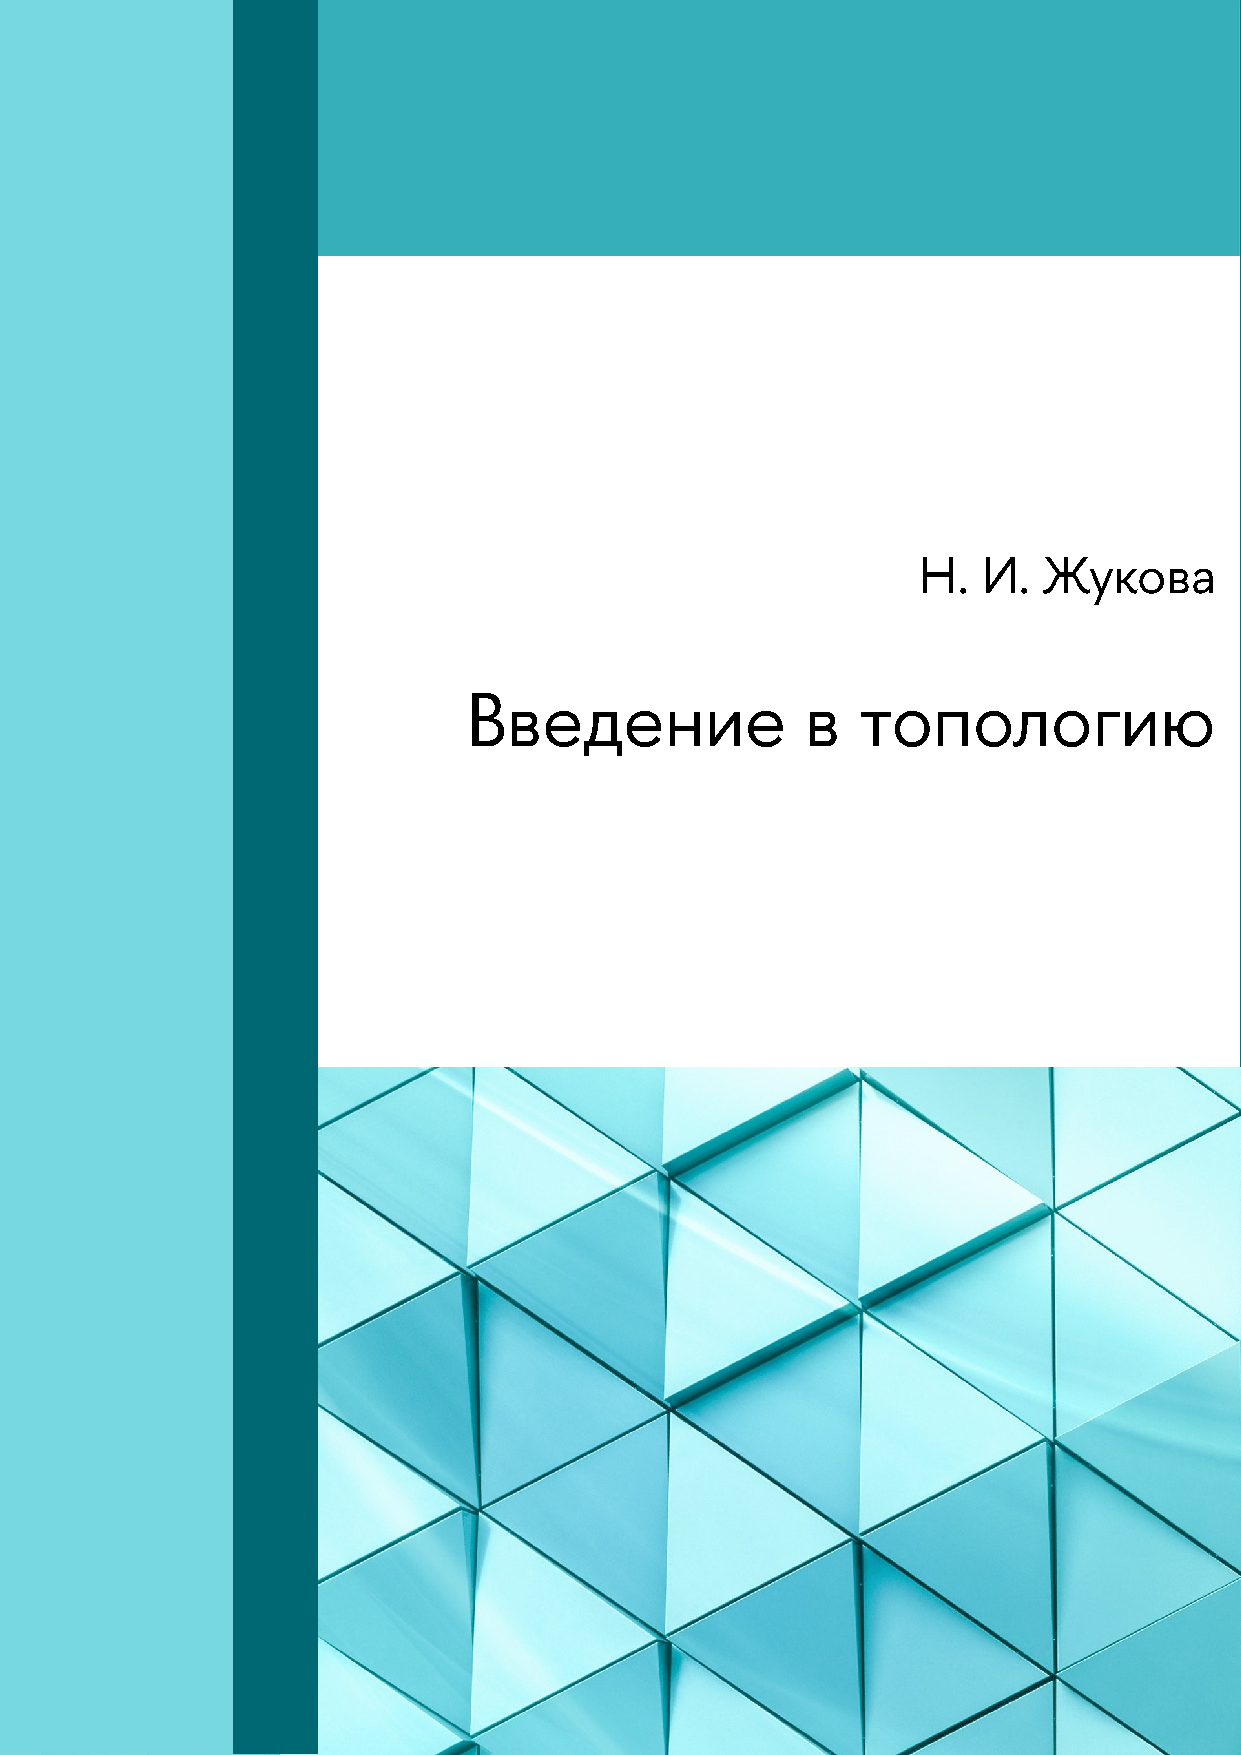
\includegraphics{pictures/folio.pdf}
%\end{figure}
%\restoregeometry
%\clearpage
%\maketitle
\tableofcontents
\newpage
%Семинар Шубина 05.09.2022
%\chapterimage{head2.png} % Chapter heading image		
%\chapter{Введение в топологию}
\chapter{Ряды}
В данном разделе мы будем изучать следующие объекты:
\begin{itemize}
    \item Числовые ряды
    \item Функциональные ряды (в т.ч. степенные, ряды Фурье)
\end{itemize}

\section{Числовые ряды}
\subsection{Базовые определения и теоремы}
\begin{defin}
Ряд - сумма счетного числа слагаемых: $$\sum_{n=1}^{\infty} a_n =a_1+a_2+
\ldots$$
\end{defin}
\begin{defin}
Частичная сумма $S_n$ - сумма первых n слагаемых
\end{defin}
\begin{defin}
Сумма ряда - предел последовательности частичных сумм 
$$S=\lim\limits_{n \to \infty}S_n$$
\end{defin}
Если предел существует и конечен, то ряд сходится. Если предел бесконечен, ряд 
расходитс. Заметим, что, согласно теоремам о пределе суммы последовательностей
и пределе последовательности, умноженной на число, сходящиеся ряды образуют
линейное пространство относительно сложения и умножения на константу.
\begin{defin}
Остаток ряда - разность между частичной суммой ряда и самим рядом: 
$$R_k=S-S_k=\sum_{n=k}^{\infty} a_k$$
\end{defin}
\textbf{Пример.} Геометрический ряд $a+aq+aq^2+\ldots$. По школьной 
формуле $S_n=\frac{1-q^n}{1-q}$. Имеем случаи:
\begin{enumerate}
    \item $|q|<1:~S=\frac{a}{1-q}$ 
    \item $|q|>1:~S=\infty$
    \item $q=1:~S=\infty$
\end{enumerate}
Итак, ряд сходится, только если $|q|<1$.\\
Следующие теоремы устанавливаются для любых рядов:
\begin{theor}(необходимое условие сходимости ряда)\\
Если ряд сходится, то предел общего члена равен 0.
Равносильная формулировка: если
$\lim\limits_{n\to\infty} a_n\ne0$, то ряд $\sum\limits_{n=1}^{\infty} a_n $
расходится.
\end{theor}
\textbf{Доказательство.} По условию, существует число $S$ - предел частичных 
сумм ряда.
Тогда $\lim\limits_{n \to \infty}a_n=\lim\limits_{n \to \infty}(S_{n}-S_{n-1})
=S-S=0$. 
$\square$

\textbf{Пример.} $\sum\limits_{n=1}^{\infty} \sin{nx},~x\ne\pi k,~k 
\in\mathbb{Z}$. 
Зафиксируем $x$. Допустим, что $\lim\limits_{n \to \infty}\sin nx=0 $. 
Но это противоречит тому, что $\sin^2(x)+\cos^2(x)=1$. Значит, ряд расходится.

\textbf{Пример.} Гармонический ряд расходится, т.к. расходится 
последовательность частичных сумм: 
$S_{2^n}>1+\frac{1}{2}+2\cdot \frac{1}{4}\ldots=1+\frac{n}{2}$
\begin{theor} (критерий Коши сходимости ряда)\\
Ряд $\sum\limits_{n=1}^{\infty} a_n$ сходится тогда и только тогда, когда
$$\forall\varepsilon>0~\exists N(\varepsilon)~\forall n>N~\forall p\in
\mathbb{N}:|a_{n+1}+\ldots+a_{n+p}|<\varepsilon$$
\end{theor}
\textbf{Доказательство.} По определению, ряд сходится, когда существует предел
частичных сумм. Применим к ним критерий Коши, получим условие: 
$|S_{n+p}-S_n|<\varepsilon$. Но $S_{n+p}-S_n\equiv a_{n+1}+...+a_{n+p}$.
$\square$ 
\begin{theor} (критерий сходимости через остаток)\\
    1. Если ряд сходится, то сходится любой из его остатков.\\
    2. Если хотя бы один остаток сходится, то ряд тоже сходится.
\end{theor}
\textbf{Доказательство.}
1. По условию, существует сумма ряда $S$. Зафиксируем номер $N\in\mathbb{N}$ и 
рассмотрим остаток $R_N=\sum\limits_{k=N+1}^{\infty} a_k$, а также 
последовательность $\sigma$ частичных сумм ряда-остатка $R_N$: 
$\sigma_n=a_{N+1}+...+a_{N+n}=\sum\limits_{k=N+1}^{N+n} a_k$.
Рассмотрим её предел:
$\lim\limits_{n \to \infty} \sigma_n=\lim\limits_{n \to \infty}(S_{n+N}-S_N)
=S-S_N=R_N$. Значит, остаток сходится.\\
2. По условию, существует такой номер $n_0$, что остаток $R_{n_0}$ сходится.
Тогда существует предел частичных сумм $\sigma_n$ этого остатка:
$\lim\limits_{n \to \infty}\sigma_n=\sigma$, 
$\sigma_n=a_{n_0}+\ldots+a_{n_0+n}$. Пусть $n_0+n=m$, тогда
$\lim\limits_{n \to \infty}S_m=\lim\limits_{n \to \infty}
(S_{n_0}+\sigma_{m-n_0})=S_{n_0}+\sigma$, то есть основной ряд сходится.
$\square$ 





%\textbf{Пример.} $\sum_{n=1}^{\infty} (\sqrt{n+2} -2\sqrt{n+1} +\sqrt{n} )$.
%Введем $a_n=b_{n+1}-b_n,~b_n=\sqrt{n+1}-\sqrt{n}$ 
%Итак, $S=\lim_{n \to \infty}$.\\
%\textbf{Пример.} $\sum_{n=1}^{\infty} \frac{n}{2^n}=2$
%\subsection{Знакопостоянные ряды}
%Докажем несколько теорем о свойствах знакопостоянных рядов.







% Продолжаем топологию 15/09/2022
\section{База топологии}
\begin{defin}
    Пусть $(X,\tau)$ - топологическое пространство
    Семейство  $\Sigma=\{W_\beta\subset X\mid \beta\in B \} $ - база топологии,
    если удовлетворяет двум условиям:\\
    1. $\Sigma\in\tau~\forall W_\beta\in\Sigma$
    2. Любое открытое подмножество Х можно представить в виде
    объединения некоторых подмножеств из $\Sigma$: 
    $\forall U\in\tau\exists W_\alpha\in\Sigma,~\alpha\in A\subset B:
    U=\Cup\limits_{\alpha\in A}W_\alpha $
\end{defin}
\textbf{Пример}. В обычной (евклидовой) топологии множество 
$\Sigma=\{D_r(a)\mid a\in\mathbb{R}^n,r>0\}$ является базой топологии.
Действительно, проверим аксиомы:\\
1. Открытая окрестность открыта.\\
2. По определению обычной топологии,каждая точка в открытом множестве
содержится в нем с некоторой окрестностью. Значит, объединение этих
окрестностей дает это множество. Более формально,
$\forall u\in\tau,\forall x\in U\Rightarrow \exists D_{\varepsilon_x}(x):
D_{\varepsilon_x}(x)\in U$. Очевидно доказывается. что 
$$\boxed{\bigcup_{x\in U}D_{\varepsilon_x}(x)=U}$$ 
\textbf{Замечание.} Если к базе добавить произвольное открытое множество, то
новое множество также будет базой.\\
\textbf{Упражнение.} Привести пример двух баз евклидовой топологии на 
плоскости, которые не пересекаются с обычной базой (открытых шаров). 
(Решение: например, база из открытых квадратных или звездчатых окрестностей).\\
\textbf{Пример.} В $(\mathbb{R}^2,\tau_{MN})$, 
$\Sigma_{MN}=\{(b,b^*)\mid b\in\} $ !!!!!!!!!!!!!!!!!!!!!\\
\textbf{Пример.} Топология ираациональных точек на прямой
$(\mathbb{R},\tau_{im}),~\tau_{im}=\{\varnothing,\mathbb{R}\}\cup
\{U\subset \mathbb{R}\setminus\mathbb{Q}\} $.
Множество иррациоанльных точек не является базой, поскольку их объединение не
содержит всю прямую. Решение: добавить саму прямую. !!!!!!!!!!!!\\

\begin{theor}
    (критерий базы в топологическом пространстве)\\
    Пусть $(X,\tau)$ - опологическое пространство, и семейство множеств 
    удовлетворяет условию $\sigma\subset \tau$. $\Sigma$ является базой 
    топологии тогда и только тогда, когда 
    $\forall u\in\tau,\forall x\in U\exists W_{\beta_0}\in\Sigma:
    x\in W_{\beta_0}\subset U$
\end{theor}
\textbf{Доказательство.} Пусть $\Sigma$ - база топологии. Тогда любое открытое 
множество можно представить в виде объединений множеств из базы. Значит, для
$x\in U$ найдется множество из базы, в котором лежит $x$.  \\
Обратно. Множесто $\Sigma$ удовлетворяет первой аксиоме базы по определению.
Докажем выполнение второй аксиомы. Для любой точки в открытом множестве
по условию теоремы найдется окрестность из $\Sigma$, лежащая в открытом
множестве. 
!!!!!!!!!!!!!!!!!!!!!!
$\square$ 

\begin{theor}
    (критерий базы на множестве)\\
    Пусть Х - произвольное множесто, $\Sigma=\{W_\beta\subset X\mid\beta
    \in B\}$ - семейство подмножеств из Х. ЧТобы на Х существовала
    топология с данной базой, необходимо и достаточно выполнения
    двух условий:\\
    1. $X=\bigcup\limits_{\beta\in B} W_\beta$\\
    2. Для любых множеств из базы найдется множество, лежащее в их
    пересечении и содержащее произвольную точку оттуда.

\end{theor}
\textbf{Доказательство.} Необходимость. Пусть $\Sigma$ - база некотрой 
топологии (Х,т). Из акиомы базы (2) следует,что что Х есть объединение
множеств из $\Sigma$. значит, выполняется первое условие теоремы. Докажем второе 
условие. Достаточно взять пересечение двух множеств из базы. Так как 
это открытые множества, его также можно представить в виде объединения
множеств из базы, и хотя бы в одном из которых лежит фиксированная точка
(по определению объединения).\\
Достаточность. Докажем, что всевозможные объедения множеств из $\Sigma$  
является топологией. пусть это есть $\tau$. Проверим аксиомы топологии:\\
1.  Пустое множество принадлежит всему, чему надо. Все простарнство 
лежит там по условию теоремы.
3. Пусть 


$\square$ 



\section{Элементарные методы интегрирования ДУ}
\subsection{Уравнения с разделяющимися переменными}
\begin{defin}\label{ODE_razdp}
Уравнение с разделяющими переменными - уравнение вида
\begin{equation}
    \frac{dx}{dt}=f(x)g(t) 
\end{equation}
где $f,g$ непрерывны на  $x\in(a,b),~t\in(\alpha,\beta)$
\end{defin}
Как решать такие уравнения? Алгебраическая интуиция подсказывает, что надо 
перенести 
дифференциалы к своим функциям и проинтегрировать. Но это ещё надо обосновать.
Сделаем следующее:\\
\begin{enumerate}
    \item Найти все $x_*:f(x_*)=0$. Тогда $x=x_*$ - решение-константа. 
    \item Пусть  $x^i_*,x^j_*$ - такие, что  $f(x^i_*)=f(x^j_*)=0$ и
    $\forall x\in(x^i_*,x^j_*):f(x)\ne0$. Тогда уравнение \ref{ODE_razdp}
эквивалентно уравнению 
$$\frac{dx}{f(x)}=g(t)dt$$
Эту штуку можно проинтегрировать с обеих сторон. Результат непрерывен и не
обращается в ноль. Значит, по теореме о неявной функции найдется решение. 
$\frac{dF}{dx}=\frac{1}{x}$(решение в области $(\alpha,\beta)\times
(x^i_*,x^j_*)$).
    \item Выписать решение на каждом интервале $(x^i_*,x^j_*)$
\end{enumerate}
Других решений не существует. Почему? Допустим, существует другое решение.
Оно не может быть константой, так как все константы были получены в п.1.
Если она \\
\textbf{Пример.} Решим уравнение $\frac{dx}{dt}=0$. Решение-константа: $x=0$.
Теперь рассмотрим два интервала: $x<0$ и  $x>0$. Если  $x<0$, имеем уравнение
 $$\frac{1}{x}\frac{dxdt}{dt}=dt$$
 Интегрируем:
 $$\int\frac{dx}{x}=\int dt$$
 Получаем, что $\ln|x|=t+C$. Выражаем искомую функцию (не забыв, на каком
 промежутке мы рассматриваем функцию, и раскрыв модуль соответственно):
 $$x=-Ce^t,~C>0$$
Для интервала $x>0$ точно такой же порядок действий, только получим другой 
знак. Итак, множество решений:
$$x=Ce^t,~C\in\mathbb{R}$$
\subsection{Уравнения, приводящиеся к уравнению с разделяющимися переменными}
\begin{defin}
Уравнение, приводящееся к уранвению с разделяющмися переменными - уравнение
вида 
\begin{equation}
    \frac{dx}{dt}=f(at+bx+c) \label{ODE_privrazd}
\end{equation}
\end{defin}
Давайте решим его. 
\begin{enumerate}
    \item Введем замену $z(t)=at+bx+c$. 
    Имеем
     $$\frac{dz}{dt}=a+b\frac{dx}{dt}$$ 
     Получаем уравнение с разделяющимися переменными. 
     $$\frac{dz}{a+bf(z)}=dt$$
\end{enumerate}
\textbf{Пример.} Решим уравнение $\frac{dx}{dt}=\cos(x+t)$. Замена 
$z=x+t,~ \frac{dz}{dt}=1$. Уравнение имеет вид
$$\frac{dz}{dt}=\frac{dx}{dt}+1$$ 
Найдем $\cos{z_*}+1=0$: это, очевидно, $\pi+2\pi k,~k\in \mathbb{Z}$ 
Свели задачу кпрошлому пункту
\subsection{Однородные уравнения}
Сначала докажем, что два определения однородного уравнения эквивалентны.
\begin{defin}\label{ODE_odn}
Однородным называется уравнение вида
\begin{equation}%\label{ODE_odn1}
    \frac{dx}{dt}=f\left(\frac{x}{t}\right) 
\end{equation} 
\end{defin}
Это уравнение инвариантно относительно замены $x\mapsto kx,~t\mapsto kt$.
Геометрически это означает, что совокупность интегральных кривых инвариантно
относительно преобразования $\theta(x,y)=(kx,ky)$.
Из этого следует, что если мы найдем одно решение, то мы найдем всю 
совокупность ему подобных. %Вставить картинку.
\begin{defin}
    (вспомогательное)\\
Уравнение в форме дифференциалов:
    $M(x,y)dx+N(x,y)dy=0$.  
\end{defin}
Это таже форма, что и $\frac{dy}{dx}=f(x,y)$, поскольку 
$\frac{dy}{dx}=-\frac{M(x,y)}{N(x,y)}$. Обратно, $-f(x,y)dx+dy=0$.
Уравнение в форме дифференциалов имеет чуть большее множество решений. 
\begin{defin}\label{ODE_odn2}
Уравнение в форме дифференциалов называется однородным, если\\
$M(kx,ky)=k^nM(x,y)$\\ 
$N(kx,ky)=k^nN(x,y)$\\
n называется степенью однородности.
\end{defin}
\begin{theor}
    Определения \ref{ODE_odn} и \ref{ODE_odn2} эквивалентны. 
\end{theor}
\textbf{Доказательство.} 1 $\Rightarrow$ 2. $\frac{dy}{dx}=f(\frac{y}{x})$\\
2 $\Rightarrow$ 1. Пусть дано уравнение в форме дифференциалов. Подставим $k$.
При $x\ne 0$ имеем 
$$\frac{dx}{dy}=-\frac{k^nM(x,y)}{k^nN(x,y)}=
-\frac{M(kx,ky)}{N(kx,ky)}=-\frac{M(1,\frac{y}{x})}{N(1,\frac{y}{x})}=
f\left( \frac{y}{x} \right) $$
$\square$ \\
\textbf{Пример.} $M=x^2+y^2$\\
\textbf{Пример (№31).} Найти уравнение, решение которых - параболы с осью, 
параллельной оси ординат и касающиеся прямых $y=0,~y=x$. 
Во-первых, поймем, как выглядит уравнение такой параболы. Исходя из геометрии,
получим, что уравнение параболы, удовлетворяющее первому условию, имеет вид 
$y=ax^2+bx+\frac{b^2}{4a}$, а первому и второму - $y=ax^2+\frac{1}{2}x+
\frac{1}{16a}$. Остался один параметр $\Rightarrow$ уравнение первого порядка. 
Подставляем и хаваем ответ бесплатно:
$$y=\left(\frac{y'-\frac{1}{2}}{2x}\right)x^2+\frac{1}{2}x+\frac{2x}{16y'-8}$$ 
\textbf{Пример (№72).} Найти линии, у которых треугольники, образованные 
касательными, осью ОХ и точкой касания, имеют одинаковую сумму катетов. 
Из геометрических соображений имеем уравнение 
$$\frac{|y|}{|y'|}+|y|=b=const$$ 
Раскрываем модули. В простейшем случае имеет уравнение с разделяющимися 
переменными. 
$$\frac{dy}{dx}=\frac{y}{b-y}$$ 
Остальные уравнения такие же в принципе. Так шо это идет в дз 
Его легчайшее (и, видимо, общее) решение: $x+C=\pm b\ln{|y|}\pm y$\\
\textbf{Пример (№76).} Геометрическая интуиция не должна подводить нас. 
Вставить картинку. Есть кароч такая формула: 
$\tg\gamma=\frac{r}{r'}$





\section{Однородное уравнение}
$$\frac{dx}{dt}=f\left(\frac{x}{t}\right)$$ 
Как искать его решение? Заменой $u(t)=\frac{x}{t}$. 
Тогда уравнение перепишется в виде $\frac{dx}{dt}=\frac{du}{dt}t+u$.
В нем переемнные разделяются: $\frac{du}{f(u)-u}=\frac{dt}{t}$. 
Итак, типы уравнений:
\begin{enumerate}
    \item С разделяющимися переменными
    \item Приводящиеся к виду $\frac{dx}{dt}=f(ax+bx+c)$ 
    \item Првиодящиеся к виду $(a_1x+b_1t+c_1)dx+(a_2x+b_2x+c_2)dt=0$
\end{enumerate}
Подумаем, можно ли это последнее привести к однородному. Добавим условие 
$c_1^2+c_2^2\ne0$ (иначе система уже однородна). В общем, если эти 
две прямые пересекаются в точке
$(x_*,t_*)$, то можно ввести новые переменные, передвинув эту точку в начало
координат: $x\mapsto x-x_*,~t\mapsto t-t_*$. Тогда система перепишется 
без $c_1,~c_2$, и таким образом будет однородной. Если прямые не пересекаются, 
то прямые либо совпадают, либо параллельны. Тогда введем замену (для любой 
прямой) $z(t)=a_1x+b_1t+c_1$. Так как прямые параллельны, то
$\frac{a_1}{a_2}=\frac{b_1}{b_2}=k$, значит, мы можем выразить 
вторую прямую: $a_2x+b_2t+c_2=\frac{1}{k}(a_1x+b_1t+kc_2)=\frac{1}{k}(z-
c_1+kc_2)$. Уравнение приводится к виду $z(t)dx+\frac{1}{k}(z-c_1+kc_2)dt=0$.
Но у нас все равно многовато переменны. Выразим $dx$ через  $z$:
$$z(\frac{dz-b_1dt}{a_1})+\frac{1}{k}(z-c_1+kc_2)=0$$ 
Умножим на $a_1k$:
 $$kzdz=kb_1zdt-a_1zdt-a_1(kc_2-c_1)dt$$ 
Домножим на $\frac{1}{kzdt}$:
$$\frac{dz}{dt}=((b_1-\frac{a_1}{k})z-a_1(kc_2-c_1))\frac{1}{z}$$ 
Finally, уравнение с разделяющимися переменными! ПОБЕДА!
\subsection{Обобщенно-однородное уравнение}
\begin{defin}
Обобщенно-однородное уравнение - уравнение вида
$$M(x,t)dx+N(x,t)dt=0$$ 
причем $M,N$ - такие. что  $\exists n\in\mathbb{R}$: если
$x=z^n(t)$, то уравнение  $M(z^n,t)nz^{n-1}dz+N(z^n,t)dt=0$ однородно.
\end{defin}
\textbf{Пример.} Испортим однородное уравнения, чтобы сделать его 
обощенно-однородным. Роман придумал, чел харош.

Сведем и этого зверя к разделяющимся переменным. 
$$\begin{cases}
    n(kz)^{n-1}M((kz)^n,kt)=k^mM(z^n,t)nz^{n-1}\\
    N((kz)^n,kt)=k^mN(z^n,t)
\end{cases}$$ 

\subsection{Уравнение в полных дифференциалах}
Напомним, что полный дифференциал $dF(x,y)$  $C^1$-гладкой функции
равен  $\frac{\partial F}{\partial x} dx+\frac{\partial F}{\partial y}dy$.
\begin{defin}
Уравнение в полных дифференциалах - уравнение вида
$$dF(x,y)=0,~F\in C^2(\Omega),~\Omega\subset \mathbb{R}^2$$
\end{defin}
Если мы знаем саму функцию, то решение находится мгновенно: $dF(x,y)=const$.
Правда, оно неявное. Выразим  $y=y(x)$ по теореме о неявной функции.\\
\textbf{Пример.} $x^2\sin{t}dt+2x\cos{t}dx=0$\\
Уравнение является уравнение в полных дифференциалах, если существуют такие
функции, что $M=\frac{\partial F}{\partial x},~N=\frac{\partial F}{\partial y}$
\begin{theor}
    (необходимое условие представления в полных дифференциалах)\\
    $$\frac{\partial M}{\partial y}=\frac{\partial N}{\partial y}$$ 
    Достаточное условие - $M_y=N_x$ в односвязной области
\end{theor}
\textbf{Доказательство.} $\square$ \\
Как подбирать такие функции? Мы знаем, что $\frac{\partial F}{\partial x}=
M(x,y)$. Проинтегрируем это равенство по $x$. Имеем  $F=\int M(x,y)dx+
\varphi(y)$. Проделаем то же самое по переменной $y$:  $\frac{\partial F}
{\partial y}=\frac{\partial }{\partial y}(\int M(x,y)dx)+\varphi'=N(x,y)$,
откуда $\varphi=\int\left(N-\frac{\partial }{\partial y}(\int Mdx) \right)dy$.
Чтобы проверить себя при решении, помним, что $\varphi$ не зависит от $x$!
Итак,
$$F=\int M(x,y)dx+\int\left(N-\frac{\partial }{\partial y}\left(\int Mdx
\right)\right)dy$$
\subsubsection{Геометрический смысл решения уравнения в полных дифференциалах}
Так как $z=z(x,y)$ - какая-то поверхность, то запись  $z=const$ - это линии
уровня, которые можно спроецировать на плокость переменных и получить 
интегральные кривые.\\
\textbf{Пример (модель Лотки-Вольтерра).} Пусть $x(t)$ - плотность карасей,
 $y(t)$ - плотность щук в некотором пруду. Щуки сдерживают рост карасей,
но от количества карасей зависит также и количество щук. Запишем систему:
$$\begin{cases} \label{lotka_volterra}
    \dot{x}=x(a-by)\\
    \dot{y}=y(-c+ex)
\end{cases}$$
Лотка придумал эту систему для биоценозов, а Вольтерра - для химических
реакций.\\
Давайте решим эту систему. Её расширенное фазовое пространство, вообще говоря,
трехмерное, поэтому будем рассматривать фазовые кривые - проекции интегральных 
на плоскость независимых параметров. Они ориентированы в направлении роста
параметра $t$. Найдем эти кривые, найдя решение уравнения 
$\frac{dy}{dx}=\frac{dy /dt}{dx /dt}=\frac{-cy+exy}{ax-bxy}$. 
Переменные разделяются: $$\frac{(a-by)dy}{y}=\frac{(-c+ex)dx}{x}$$ 
Представим его в полных дифференциалах: 
$$d\left( a\ln y-by+c\ln x -ex \right)=0$$
Значит, решение имеет вид $a\ln y-by+c\ln x-ex=h=const$.
Выглядит очень сложно, но давайте попробуем построить изолинии. 
Введм функцию $F=\ln{(y^ax^c)}-by-ex$, и поищем её изолинии. Сначала найдем
критические точки: $(x_*,y_*)=(\frac{c}{e},\frac{a}{b})$ (получилась 
единственная точка). Определим тип критической точки (составим гессиан, 
посчитаем его знакоопределенность); получим, что это точка максимума.
Линии уровня - какие-то окружности/эллипсы.\\
\begin{figure}[H]
    \centering
    \input{figures/Lotka-Volterra.pdf_tex} %для pdf_tex
    %\includegraphics{}  % для png, pdf
    \caption{Первый интеграл системы Лотки-Вольтерры}
    \label{fig:}
\end{figure}
\textbf{Упражнение.} Доказать, что фазовые кривые замкнуты.

\textbf{Доказательство (\cite{Arnold},\S 2.7).} Так как 
$\frac{dF}{dt} = 0$, то функция $F$ сохряняется вдоль фазовых кривых. 
Иначе говоря, фазовые кривые являются изолиниями фунции $F$. Но 
график  $F$ является суммой двух <<холмов>>, образованных логарифмами, 
и поэтому сам является холмом. Посколько изолинии холма - замкнутые кривые,
то и фазовые кривые системы Лотки-Вольтерры замкнуты. $\square$\\
Теперь нам надо понять, куда закручиваются эти линии, как они ориентированы.
Они закручиваются против часовой стрелки вокруг критической точки, кстати,
область решения - первая координатная четверть. Чтобы избежать проблем с 
дискретностью, наши переменные - это плотность населения пруда. 

 



%Гомеоморфный (без самопересечений, так как биекция) образ окружности в
%плоскости можно непрерывно продеформировать в точку. Теорема Жордана: 
%гомеоморфный образ окружности делит плоскость на две компоненты связности. 
%Теорема Шёнфлиса: внутренняя часть этой плоскости гомеоморфна открытому 
%диску. Это кстати эквивалентно тому, что фундаментальная группа 
%тривиальна. 

\begin{defin}
Автономное ДУ - дифференциальное уравнение, правая часть которого не зависит
от времени.
\end{defin}
Автономные уравнения не могут быть динамическими системами, так как они 
не зависят от времени, но можно искусственно этого достичь.\\
\textbf{Пример.} Нелинейный консервативный
осциллятор. Рассмотрим маятник с координатами
$\varphi$ - отклонение от положения равновесия. Рассмотрим плоские
колебания маятника массой $m$ и длиной $l$. При повороте на малый угол 
движение можно представить как прямолинейное движение по касательной.
Запишем второй закон Ньютона в проекции на касательную: 
$$\vec\tau:~m\frac{d^2x}{dt^2}=-mg\sin\varphi$$ 
Пусть $\Delta x$ - длина дуги окружности, примерно равная малой части 
касательной. Тогда  $\Delta x=l\Delta\varphi+o(\Delta\varphi)$.
Получим уравнение
$\frac{fx}{dt}=l \frac{d\varphi}{dt}$. Finally,
$$ml \frac{d^2\varphi}{dt^2}=-mg\sin\varphi$$ 
- уравнение колебания маятника. Оно нелинейное из-за синуса. 
Оно имеет порядок 2, значит, нам надо
зафиксировать начальные условия: $\varphi(0),~\dot\varphi(0)$.
Уравнение тогда превратится в систему
$$\begin{cases}
    \dot\varphi=\psi\\
    \dot\psi=-\omega^2\sin\varphi
\end{cases}$$
Кстати, если мы напишем функцию Лагранжа и напишем уравнение Лагранжа для
него, то получим это же уравнение.\\
Начнем решение. Сделаем замену $\dot\varphi=\psi$. Теперь введем фазовое 
пространство угол-скорость таким образом, чтобы близкие точки были близки.
В угловых координатах мы склеим точки $\pi,-\pi$ у координат углов (точнее,
создадим факторпространство по отношению $(\varphi,\psi)\sim(\varphi+2\pi k,
\psi)$). Получим, что фазовое пространство - цилиндр. Любая замкнутая кривая 
- это некоторая траектория (вообще говоря, определляемая уравнением).
На цилиндре есть два типа замкнутых кривых - стягиваемые в точку и 
нестягиваемые. Вторые отвечают за движение через верх. \\
Продолжаем решение. Из системы имеем 
$\frac{d\psi}{d\varphi}=-\frac{\omega^2\sin\varphi}{\psi}$.
Полная энергия равна константе:
$\frac{m\psi^2}{2}+\frac{mg}{l}(1-\cos\varphi)=h$.
Это мы вывели из формы уранвения в полных диференциалах. 
В общем, решаем. Получим
$$\varphi=\pm\sqrt{\frac{2}{m}\left( h-\frac{mg}{l}(1-\cos\varphi) \right) }$$ 
Нарисуем фазовые траектории, и ещё функцию 
$F(\varphi)=\frac{mg}{l}(1-\cos\varphi)$.
Уровни постоянной энергии - одномерные торы. Как и обычно с функцией
Гамильтона. 
Из анализа фазовых траекторий можно выяснить, что период колебаний растет по
мере увеличения энергии. Также есть два состояния равновесия: верхнее 
(неустойчивое) и нижнее (устойчивое). 










%Лекция 13.10.22
\section{Уравнения и ряды Тейлора}
Пусть $\frac{dx}{dt}=f(t,x)$. Рассмотрим $x(t_0)=x_0$. Разложим в ряд
Тейлора: $x(t)=x(t_0)+\frac{dx}{dt}(t_0)(t-t_0)+o(t-t_0)$.
Отбросив члены высшего порядка (прямо как топовые физики), получим 
приближенное решение. Приближенные решение можно итерировать, и это
будет широко известный \textbf{метод Эйлера} (первого
порядка). $t_{k+1}=t_k+h,~x_{k+1}=x_k+f(t_k,x_k)h$ 

\section{Практика}
\textbf{Пример (№111)}. $(y+\sqrt{xy})dx=xdy$. Уравнение однородно (
проверим умножением на $k$). Значит, делаем замену $u(x)=\frac{y}{x}$.
Имеем $dy=u\cdot dx+du\cdot x$. Переменные разделяются: 
$\frac{dx}{x}=\frac{du}{\sqrt{u}}$\\
\textbf{Пример (№113)}. $(2x-4y+6)dx+(x+y-3)dy$. Переносим начало координат
в точку пересечения.\\
\textbf{Пример (№126)}. $y'=y^2-\frac{2}{x^2}$. Это - обобщенно-однородное
уравнение, то есть приводится к однородному заменой $y=z^m(x)$.
$y'=mz^{m-1}z$ Далее
$mz^{m-1}z=z^{2m}-\frac{2}{x^2}$ 
Теперь уравнение однородно. Введем замену $\frac{z}{x}=u,~z=ux$.
Получим $u'x+u=-1+2u^2$\\
\textbf{Пример (№128)}. $\frac{2}{3}xyy'=\sqrt{x^6-y^4}+y^2$. 
Пусть $y=z^m$. Идея: сделать так, чтобы под корнем степень у $x$ и $y$ была
одинаковой.\\
\textbf{Пример (№)} $2xydx+(x^2-y^2)dy=0$. Подберем функцию, полным 
дифференицалом которого является это выражение; получим  $F(x,y)=
x^2y-\frac{1}{3}y^3$. Решние: $F=C=const$\\
\textbf{Пример (№192)}. $(1+y^2\sin{2x})dx-2y\cos^2{x}dy$. Мы должны 
показать, что вторые производные равны. Тогда это значит, что
$F_{xy}=F_{yx}$, и такая функция вообще существует на некотором диске
(где правая часть не обращается в ноль). Интегируем два раза, и найдем эту
функцию: $F(x,y)=x-y^2 \frac{1}{2}\cos{2x}-\frac{y^2}{2}+C_0$.
Итак, ответ: $\boxed{F=const}$ \\
\textbf{Пример (№202)}. $y^2dx+(xy+\tg{xy})dy=0$. Является ли однородным,
в полных дифференциалах? Давайте раскроем скобки и сгруппируем:
$y(ydx+xdy)+\tg{xy}dy$. Это то же, что и  $\frac{d(xy)}{\tg{xy}}+\frac{dy}{y}
=0$. Домножим на $\frac{1}{y\tg{xy}}$ и хаваем уравнение в полных 
дифференицалах бесплатно. То, на что домножили - интегрирующий множитель.















\begin{theor}
    (признак Абеля равномерной сходимости функционального ряда)\\
Дан ряд $\sum\limits_{n=1}^{\infty} a_n(x)b_n(x)$ и $\forall x\in X$:\\
1. $|a_n(x)|\leqslant M=const$ для всех $n$;\\
2.  $\{a_n(x)\} $ мнонотонна;\\
3. $\sum\limits_{n=1}^{\infty} b_n(x)$ равномерно сходится на $X$;\\
Тогда исходный ряд равномерно сходится на  $X$.
\end{theor}
\textbf{Доказательство.}  По определению Коши. Фиксируем $\varepsilon>0$.
Так как ряд с общим членом $b_n$ сходится равномерно, то по критерию Коши для
$$\frac{\varepsilon}{3M}>0~\exists n_0(\varepsilon)~\forall n>n_0~\forall p\in
\mathbb{N}~ \forall x\in X:\left|\sum\limits_{k=n+1}^{n+p} b_k(x)\right|<
\frac{\varepsilon}{3M}$$ Тогда по неравенству Абеля 
$$\left|\sum\limits_{k=n+1}^{n+p} b_k(x)a_k(x)\right|\leqslant 
\frac{\varepsilon}{3M}(|a_{n+1}|+2|a_{n+p}(x)|)<\frac{\varepsilon}{3M}\cdot 
3M=\varepsilon$$
Тогда по критерию Коши этот ряд сходится равномерно на $X$. $\square$ 

\textbf{Пример.} Исследуем на равномерную сходимоcть ряд 
$\sum\limits_{n=1}^{\infty} \frac{\cos{nx}\sin{x}arctg{nx}}{\sqrt{n^2+x^2}}$. 
Алгоритм:\\
1. Арктангенс монотонен и ограничен.\\
2. Все остальное сходится по Дирихле.
\subsection{Свойства равномерно сходящихся рядов}
\begin{theor}
    (о непрерывности суммы равномерно сходящегося ряда)\\
    Дан ряд $\sum\limits_{n=1}^{\infty} a_n(x)$, причем \\
    1. Все функции непрерывны на множестве $X$;\\
2. $\sum\limits_{n=1}^{\infty} a_n(x)$ сходится равномерно к $S(x)$ на $X$;\\
Тогда $S(x)$ непрерывна на $X$. 
\end{theor}
\textbf{Доказательство.}  По условию, сумма из  $a_n(x)$ сходится равномерно
на  $X$ к  $S(x)$, то есть  $S_n(x)\rightrightarrows S(x)$ на  $X$, 
$S_n(x)$ непрерывна как сумма. Тогда по теореме о непрерывности предела
равномерно сходящейся последовательности, составленной из непрерывных
функций,  $S(x)$  непрерывна. Другая формулировка:  
$$\lim\limits_{x\to x_0}\sum\limits_{n=1}^{\infty} a_n(x) =
\sum\limits_{n=1}^{\infty}\lim\limits_{x\to x_0} a_n(x)
$$
(то есть можно поменять местами сумму и предел). $\square$ 

\textbf{Пример.} $\sum\limits_{n=1}^{\infty} \frac{\sin{nx}}{n}=f(x)$ - 
непрерывна на $(0,2\pi)$
\begin{theor}
(об интегрировании равномерно сходящегося ряда)\\
Пусть дан ряд $\sum\limits_{n=1}^{\infty} a_n(x)$, причем \\
 1. все функции непрерывны на отрезке $[a,b];$\\
 2. $\sum\limits_{n=1}^{\infty} a_n(x)$ сходится равномерно на $[a,b]$ к $s
 (x)$;\\
 Тогда $$\forall x,x_0\in[a,b]:~\int\limits^x_{x_0}\left( \sum\limits_{n=1}^
 {\infty} a_n(t) \right)dt=\sum\limits_{n=1}^{\infty} \left( 
\int\limits_{x_0}^{x}a_n(t)dt \right) $$ 
 (можно менять интеграл и сумму).
\end{theor}
\textbf{Доказательство.} Докажем, что $\int\limits^x_{x_0}S(t)dt=\sum\limits_{n=1}^{\infty} \int\limits^x_{x_0}a_n(t)dt$. По предыдущей теореме $S(t)$ 
непрерывна на  $[a,b]$, значит,интегрируема на нем по Риману. 
Обозначим  $\sigma_n(x)=\sum\limits_{k=1}^{n}\int\limits^x_{x_0}a_k(t)dt$ и
докажем, что $\sigma_n(x)\rightrightarrows\int\limits^x_{x_0}S(t)dt$.\\
Зафиксируем $\varepsilon>0$. По условию, $S_n(t)$ равномерно сходится на 
$[a,b]$ для  
$$\frac{\varepsilon}{b-a}>0~\exists n_0(\varepsilon)~\forall 
n>n_0~\forall x\in[a,b]:|S_n(t)-S(t)|<\frac{\varepsilon}{b-a}$$
Тогда
$\left|\sigma_n(x)-\int\limits^x_{x_0}S(t)dt\right|=
\left| \sum\limits_{k=1}^{n} \int\limits_{x_0}^{x} a_k(t)dt-
\int\limits_{x_0}^{x}S(t)dt\right|=\left| \int\limits_{x_0}^{x}(S_n(t)-S(t))dt
\right|\leqslant \left| \int\limits_{x_0}^{x}|S_n(t)-S(t)|dt\right| 
<\frac{\varepsilon}{b-a}\cdot |x-x_0|<\varepsilon$.
Значит, $\sigma_n(x)\rightrightarrows \int\limits_{x_0}^{x} S_n(t)dt$.
$\square$ 
\begin{theor}
(о дифференцировании равномерно сходящегося ряда)\\
Пусть дан ряд $\sum\limits_{n=1}^{\infty} a_n(x)$, причем \\
 1. Производные всех функций непрерывны на отрезке $[a,b];$\\
 2. $\sum\limits_{n=1}^{\infty} a_n(x)$ сходится на $[a,b]$ поточечно;\\
 3. Ряд из производных сходится равномерно на $[a,b]$ к  $S(x)$;\\
 Тогда 
$$\sum\limits_{n=a}^{\infty} a'_n(x)=
\left( \sum\limits_{n=1}^{\infty} a_n \right)'$$
то есть в ряде  можно менять производную и сумму, причем 
$\sum\limits_{n=1}^{\infty} a_n$ сходится равномерно.
\end{theor}
\textbf{Доказательство.} 
1. Используем предыдущую теорему. Тогда
$$\int\limits_{x_0}^x\left( \sum\limits_{n=1}^{\infty} a'_n(t) \right)dt=
\sum\limits_{n=1}^{\infty} \int\limits_{x_0}^xa'_n(t)dt$$
Получаем, что в равенстве
$\int\limits_{x_0}^xS(t)dt=\sum\limits_{n=1}^{\infty} (a_n(x)-a_n
(x_0))$ справа стоит число (в силу непрерывности функции), ряд из $a_n(x_0)$
сходится по условию, следовательно, ряд из $a_n(x)$ сходится.
Поэтому, дифференцируя равенство 
$\int\limits_{x_0}^{x} \sum\limits_{n=1}^{\infty} a_n(t)\,dt=
\sum\limits_{n=1}^{\infty} a_n(x)-\sum\limits_{n=1}^{\infty} a_n(x_0)$,
получаем первое утверждение теоремы.

Теперь покажем равномерную сходимость исходного ряда. 
Для этого покажем, что остаток 
ряда из производных $r_n(x)=\sum\limits_{k=n+1}^{\infty} a'_n(x)$
равномерно стремится к нулю. 
Из этого следует применимость теоремы об инетгировании: 
$\int\limits_{x_0}^{x}\sum\limits_{k=n+1}^{\infty} a'_k(t)\,dt=
\sum\limits_{k=n+1}^{\infty} \int\limits_{x_0}^{x} a'_k(t)dt=
\sum\limits_{k=n+1}^{\infty} (a_k(x)-a_k(x_0))$. Если ряд удовлетворяет 
теореме об интегрировании, то и его остатки тоже, значит,
$\int\limits_{x_0}^{x} r_n(t)dt=R_n(x)-R_n(x_0)$, откуда
$$R_n(x)=\int\limits_{x_0}^{x} r_n(t)dt+R_n(x_0)\quad(1)$$.
Зафиксируем $\varepsilon>0$. По условию, остаток обычного ряда стремится
к нулю: $R_n(x)\to0$. Тогда для 
$$\frac{\varepsilon}{2}>0~\exists n_1
(\varepsilon)~\forall n>n_1:|R_n(x_0)|<\frac{\varepsilon}{2}$$
Остаток ряда из производных равномерно стремится к нулю, тогда
для 
$$\frac{\varepsilon}{2(b-a)}>0~\exists n_2(\varepsilon)~\forall n>n_2~
\forall x\in[a,b]:|r_n(x)|<\frac{\varepsilon}{2(b-a)}$$
По формуле (1) получаем: 
$|R_n(x)|\leqslant \left| \int\limits_{x_0}^{x} r_n(t)dt \right|+
|R_n(x_0)|\leqslant \left|\left| \int\limits_{x_0}^{x} r_n(t)dt \right|+
|R_n(x_0)| \right|<\frac{\varepsilon}{2(b-a)}\cdot |x-x_0|+
\frac{\varepsilon}{2}=\varepsilon$. $\square$ 



\begin{defin}
Функция $\tilde x(t)$ определенная на интервале $(a,b)$, называется 
продолжением решения вправо, если она совпадает с $x(t)$ на некотором
подинтервале.
\end{defin}

\begin{theor}
    (о продолжении решения)\\
    Пусть дано уравнение $\frac{dx}{dt}=f(t,x),~x(t_0)=x_0$, 
    функции $f(t,x),~\frac{\partial f}{\partial x}$ непрерывны на компакте
    $D\subset \mathbb{R}^2$ (причем в $D$ лежит как минимум 1 шар),
    $x(t,t_0,x_0)$ - решение задачи Коши для  $(t_0,x_0)\in Int D$. 
    Тогда существует решение, определенное на отрезке $[a,b]$, причем
     $(a,\tilde x(a,t_0,x_0)),(b,\tilde x(b,t_0,x_0))\in \partial D$.
     Иначе говоря, решение продолжается на границу компакта.
\end{theor}
\textbf{Доказательство.} В силу теоремы о существовании и единственности 
решения, функция $(x,t_0,x_0)$ определена на отрезке $[t_0-\delta_0,
t_0+\delta_0]$, где $\delta_0=\frac{r_0}{\sqrt{1+m^2} }= \frac{\rho(P_1,
\partial D)}{\sqrt{1+m^2} }$. 

Положим $t_1=t_0+\delta_0,~x_1=x(t_1,t_0,x_0),p_1(t_1,x_1)$. 
определим 
$$\tilde x(t,t_0,x_0)=\begin{cases}
    x(t,t_0,x_0),~t\in [t_0-\delta_0,t_0+\delta_0];\\
    x(t,t_1,x_1),~t\in [t_1-\delta_1,t_1+\delta_1];
\end{cases}$$
Если $(x_1,t_1)$ лежит на границе, то все хорошо. Если нет, то будем 
увеличивать шар, пока не достигнем границы множества (в силу компактности 
это всегда можно сделать). 

Возможен вариант, когда последовательность $\delta_i$ стремится к нулю и 
сама не затрагивает границу компакта. Рассмотрим функцию, определенную 
на $t\in [t_0-\delta_0,t+k+\delta_k]$. Последовательность 
$t_k$невозрастающая и ограниченная, поэтому существует и предел 
$b$. Функция $\tilde x$  определена на объединении интервало
$\bigcup\limits_{k}[t_0-\delta_0,t_k+\delta_k]=[t_0-\delta_0,b)$.
Воспользуемся непрерывностью функций: пусть $0<h\ll1$.
Тогда $\forall \alpha,\beta\in (b-h,b):|\tilde| x(\alpha,t_0,x_0)-
\tilde x(\beta,t_0,x_0)|\leqslant m|\alpha-\beta|<mh$. 
Последовательность $\tilde x_k$ фундаментальна, значит по критерию Коши 
у неё есть конечный предел. Положим этот предел значением функции 
в точке $b$:  $x^*=\tilde x(b)$. Тогда функция непрерывна на $[t_0-\delta_0,
b]$. Вспомним про интегральное уравнение: заметим, что $\tilde(x)$ 
удовлетворяет интегральному уравнению на интервале. Функция, дополненная
на конце интервала, непрерывна и также удовлетворяет интегральному 
уравнению, поэтому в ней есть и производная (по эквивалентности
определений).

Покажем, что точка $b$ лежит на границе области  $D$. Предположим противное,
тогда она лежит во внутренности $D$. Тогда она лежит в нем вместе
с некоторой $2\varepsilon$-окрестностью с центром в $p^*=(t^*,x^*)$.
Так как точки $p\to p^*$, то  все $p_i,i>k$ лежат в  $\varepsilon$-шаре
точки $p^*$. Тогда расстояние до границы больше  $\varepsilon$, 
и мы получаем противоречие с тем, что ряд из $\delta_k$ сходится и также
удален от границы больше чем на $\varepsilon$. Значит, $p^*\in \partial D$.
$\square$ \\
\textbf{Следствие.} Пусть $D\subset \mathbb{R}^2$ - такое неограниченное 
замкнтуое 
подмножество плоскости, что для любых $(a,b):D_{a,b}=D\cap \{
(t,x):a\leqslant t\leqslant b\}$ компактно, функции 
$f(t,x),\frac{\partial f}{\partial x}$ непрерывны на $D$. Тогда 
решение задачи Коши продолжается либо неограниченно, либо до выхода на границу
 $D$. Доказать самостоятельно. 

\textbf{Пример.} $x'=t^3-x^3$. Показать, что любое решение этого
уравнения продолжается неограниченно вправо.  Нарисуем изоклину $x=t$. 
Заметим, что если $t_0>x_0$, то $x(t,t_0,x_0)\in D:$. Тогда в силу следствия
решение продолжается на границу, на граница не достигается, то есть

\textbf{Пример.} $x'=1+x^2$. 
Его решение - $x=\tg(x+C),~C=\arctg(x_0)-t_0$, 
поэтому его нельзя продолжить до бесконечности,
так как каждое решение определено на конечном интервале $(C_0-\frac{\pi}{2},
C_0+\frac{\pi}{2})$. 

%\textbf{Практика.}
\subsection{Практика}

\textbf{Пример (№199).} $y^2dx-(xy-x^3)dy=0$. Раскроем скобки и перегруппируем
слагаемые: $y(ydx-xdy)-x^3dy=0$. Поделим все на  $x^2$, тогда получим:  
$-d\left( \frac{x}{y}-\frac{x}{y}dy=0 \right)$. Домножая на $- \frac{y}{x}$,
получаем $d\left( \frac{1}{2}\left( \frac{y}{x} \right)^2  \right) +dy=0$.
Итак, $d\left( \frac{1}{2}\left( \frac{y}{x} \right)^2 +y\right)=0$
В общем, мы нашли интегрирующий множитель методом внимательного взгляда. 
Ответ: $\frac{1}{2}\left( \frac{y}{x} \right)^2+y=const$.

\textbf{Пример (№202).} $d(\ln|\sin(xy)|)+\ln|y|=0$.

\begin{defin}
Интегрирующий множитель - такая функция $\mu(z(x,y))$, что при домножении на 
неё уравнение становится уравнением в полных дифференциалах.
\end{defin}
Тогда $\frac{\partial(\mu M)}{\partial y}=\frac{\partial(\mu N)}{\partial x}$.
То есть $\frac{\partial \mu}{\partial z}\frac{\partial z}{\partial y}M=
$
Получаем, что $\frac{d\mu}{\mu}= \frac{N_x-M_y}{z_yM-z_xN}=P(z)$. То есть, если
интегрирующий множитель существует, то он удовлетворяет этому условию. 
Значит, $\mu=e^{\int\limits_{}^{} P(z)dz}$.

\textbf{Пример (№212).} $(2x^2y^3-1)ydx+(4x^2y^3-1)xdx=0$.
Пусть $z=xy$. Найдем интегрирующий множитель: $\mu=\frac{1}{(xy)^2}$.



%Лекция 17.11.22
\subsection{Ряды Тейлора}
\begin{defin}
Пусть в некоторой окрестности $U(x_0)$ существуют производные всех порядков
у функции. Тогда для функции $y=f(x)$ в точке $x_0$ существует ряд Тейлора:
$$f(x_0)=\sum\limits_{n=1}^{\infty} \frac{f^{(n)}(x_0)}{n!}(x-x_0)^n$$
\end{defin}
Если $x_0=0$, то ряд называется рядом Маклорена.
\begin{theor}
Если функция представляется в виде степенного ряда, то он совпадает с 
её рядом Тейлора. $f(x)=\sum\limits_{n=1}^{\infty} c_n(x-x_0)^n$.
\end{theor}
\textbf{Доказательство.}  Пусть $(x_0-R,x_0+R)$ - интервал сходимости ряда. 
Из разложения функции в ряд имеем  $f(x_0)=c_0$. Беря производную, получаем,
что  $f'(x_0)=c_1$. Дифференцируя дальше, получаем, что  $c_n=
\frac{f^{(n)}(x_0)}{n!}$. $\square$ \\
Если по произвольной функции составить ряд Тейлора, то совсем не обязательно,
что он сойдется к этой функции. Сейчас поясним:\\
\textbf{Пример.} Рассмотрим
$$f(x)=\begin{cases}
    e^{-\frac{1}{x^2}},~x\ne0\\0,~x=0    
\end{cases}$$
Очевидно (по индукции), что производная порядка $f^{(n)}(x)=e^{-\frac{1}{x^2}}
\cdot p\left( \frac{1}{x} \right)$, где $p(t)$ - многочлен. Посчитаем
производнуюв нуле; первая производная в нуле - ноль. По индукции получаем,
что все остальные производные тоже равны нулю. Значит, ряд Маклорена 
тождественно равен нулю, и сходится \textit{не к исходной функции, а
к тождественно нулевой}.
 \begin{theor}
     (достаточное условие сходимости ряда Тейлора)\\
Пусть $\exists h>0,~\exists M=const$ такие, что $\forall x\in \mathbb{N}~
\forall x\in(x_0-h,x_0+h): |f^{(n)}(x)|\leqslant M$. Тогда на всей
$h$-окрестности точки $x_0$ функция равна своему ряду Тейлора, 
причем он сходится равномерно на данном интервале. 
\end{theor}
\textbf{Доказательство.}  Разложим функцию $f(x)$ в ряд Тейлора и запишем  
остаток в форме Лагранжа: $r_n(x)=\frac{f^{(n+1)}(\xi)}{(n+1)!}(x-x_0)^{n+1}$,
$\xi\in(x_0,x)$ (лежит между ними).  Остаток по модуля меньше, чем
$M\cdot \frac{h^{n+1}}{(n+1)!}$ - значит, он равномерно сходится к нулю. 
Поэтому и сам ряд сходится равномерно на $(x_0-h,x_0+h)$. $\square$ 
\subsubsection{Ряды Маклорена для основных функций}
\begin{enumerate}
    \item $e^x=1+x+\frac{x^2}{2!}+...+\frac{x^n}{n!}...,~x\in\mathbb{R}$
\item $\sh(x)=x+\frac{x^3}{3!}+...+\frac{x^{2n+1}}{(2n+1)!}+...,~
x\in\mathbb{R}$
\item $\ch(x)=1+\frac{x^2}{2!}+...+\frac{x^{2n}}{(2n)!}+...,~x\in\mathbb{R}$
\item $\sin(x)=x-\frac{x^3}{3!}-...+(-1)^n\frac{x^{2n+1}}{(2n+1)!}+...,
    ~x\in \mathbb{R}$
\item $\cos(x)=1-\frac{x^2}{2!}+...+(-1)^n \frac{x^{2n}}{(2n)!}+...,~
    x\in\mathbb{R}$ 
\item $\ln(1+x)=1-\frac{x^2}{2}+\frac{x^3}{3}-...+(-1)^n
    \frac{x^n}{n}+...,~x\in(-1,1]$
\item $\ln(1-x)=,~x\in[-1,1)$
\item $\ln \frac{1+x}{1-x}=2 \sum\limits_{n=0}^{\infty} \frac{x^{2n+1}}
    {2n+1},~ x\in(-1,1)$ - в этой формуле функция примнимает все положительные
значения, поэтому она круче. 
\item $(1+x)^\alpha=1+\alpha x+...+\frac{\alpha(\alpha-1)...(\alpha-n+1)}
    {n!}x^n+...$
\item $arctg(x)=x-\frac{x^3}{3}+\frac{x^5}{5}+...+(-1)^n \frac{x^{2n+1}}
    {2n+1}+...~,x\in[-1,1]$
\item $arcsin(x)=x+\sum\limits_{n=1}^{\infty} \frac{(2n-1)!!\cdot x^{2n+1}}
    {n!*82^n(2n+1)},~x\in(-1,1)$


\end{enumerate}
(Для логарифма) покажем, что остаток ряда стремится к нулю.\\
1. $x\in[0,1]:~r_n(x)=\frac{f^{(n+1)}(\xi)}{(n+1)!}x^{n+1}$. 
Подставим $\xi=x_0+\theta(x-x_0),~\theta=\theta(x,n)$.
При этом имем оценку $0\leqslant x\leqslant 1\leqslant 1+\theta x$.
Получим
$|r_n(x)|=\frac{1}{n+1}\cdot \left( \frac{x}{1+\theta x} \right)^{n+1}
\leqslant \frac{1}{n+1}$. Значит, остаток равномерно сходится к 0 на $[0,1]$.
Чтобы доказать равномерную сходимость на  $(-1,0)$, запишем остаток в 
форме Коши. Получим  $|r_n(x)|=\left( \frac{1-\theta}{1+\theta x} \right)^n
\cdot \frac{|x|^{n+1}}{1+\theta x}$. Первая дробь меньше 1, вторую 
оценим как $\frac{|x|^{n+1}}{1-{|x|}}$, что при фиксированном $x$ стремится 
к нулю.
Значит, мы можем писать разложение для логарифма!\\
\textbf{Пример.} $\sum\limits_{n=0}^{\infty} \frac{2^n}{n!}=e^2$\\
\textbf{Ряд $(1+x)^\alpha$}. Найдем радиус сходимости:
$R=\lim\limits_{n \to \infty} |\frac{a_n}{a_{n+1}}|=|\frac{n+1}{\alpha-n}|=1$.
Запишем остаток в форме Коши: $(1+x)^\alpha=1+\alpha x+...+\frac{\alpha
(\alpha-1)...(\alpha-n+1)}{n!}x^n+r_n,~r_n(x)=\frac{f^{(n+1)}(\theta x)}{n!}
(1-\theta)^nx^{n+1}$. Если остаток стремится к нулю, то и ряд сходится к 
данной функции. Пусть $r_n=A_n\cdot B_n\cdot C_n$, где $B_n(x)=(1+\theta x)^{
\alpha-1},~C_n(x)=\left( \frac{1-\theta}{1+\theta x} \right)^n,~A_n=
\frac{\alpha(\alpha-1)...(\alpha-n)}{n!}x^{n+1}$. $A_n\to0$ по признаку 
Даламбера, $|B_n(x)|\leqslant max \{(1-|x|)^{\alpha-1},(1+|x|)^{\alpha-1}\}$,
$C_n(x)<1$, значит, остаток стремится к нулю, и ряд сходится к функции.\\
\textbf{Задача.} Доказать, что в $x=1$ ряд сходится при $\alpha>-1$,
расходится при $\alpha\leqslant -1$. В точке $x=-1$ сходится абсолютно при
 $\alpha\geqslant0$, расходится при $\alpha<0$\\
Выражения для арксинуса и арктангенса получаются интегрированием разложния
их производных. \\
Рассмотрим сходимость арксинуса на концах!!!!!!!!!!!!!!!!!!!!!!






%Первые 9 лекций - материал к коллоквиуму
\subsection{Использование степенных рядов}
Разложение функции в ряд - мощнейшая тема. Иногда вфизике и других прикладных
областях делают так:\\
\textbf{Пример.} Возьмем интеграл
$\int\limits$ 


\textbf{Пример}. Решм диффур $y''=2xy'+4y$

\end{document}
